\chapter{Signal and Background Modeling}
In each category, we carry out a shape analysis to search for a signal peak in the $m_{\ell\ell\gamma}$ spectrum.
The signal and background mass shapes are modeled using parametric functions. 

\section{Signal Modeling}
The signal model is defined as the sum of Crystal Ball~\cite{CB-Oreglia} and Gaussian functions.
The signal shape parameters are determined by fitting this model to simulated signal events in each category.
To account for differences in mass resolution, these fits are performed separately for the event samples used to model each data-taking year, as well as for muon and electron channel events.
This results in six signal models that are summed to give the total signal expectation in a given category.
Separate sets of parameter values are found by fitting simulated events with $m_\PH$ of $120$, $125$, and $130$\GeV.
Using linear interpolation, parameter values are also determined at 1\GeV intervals in $m_\PH$ from $120$--$130$\GeV, as well as at 125.38\GeV.
In the fit to data, the mean and resolution parameters are allowed to vary subject to constraints from several systematic uncertainties, described in Section~\ref{sec:uncertainties}, while the remaining parameters are held fixed. 

Figure [REF] (REF) shows the signal fits for the $m_\PH=125\GeV$ simulated samples in the electron (muon) channel for the 2016 data-taking period. Figure [REF] shows the signal fits for the lepton-tagged category for the 2016 data-taking period, in which electron and muon channel events are combined. In the lepton-tagged category, the signal shape is modeled separately for ZH and WH production in order to account for differences in potential lepton mispairing. Signal fits for the 2017 and 2018 data-taking periods are shown in Figs. [REF] in Appendix [REF].

\begin{figure}
	\begin{center}
		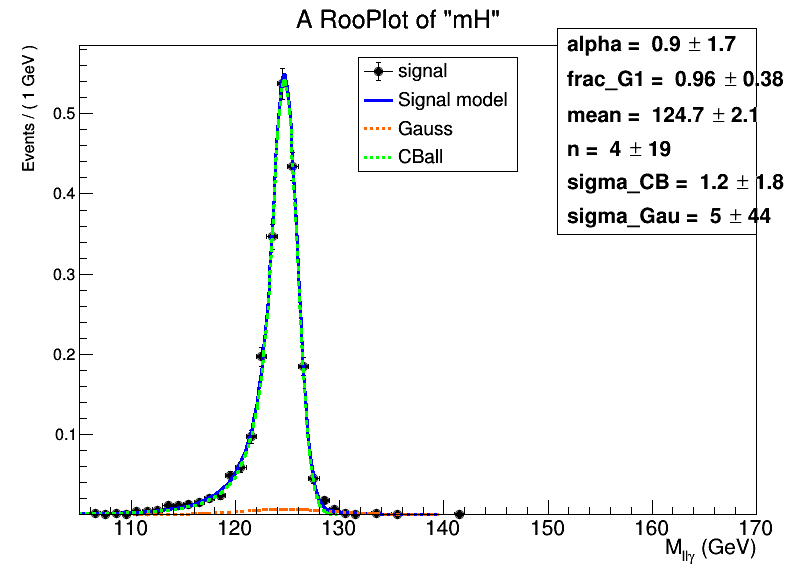
\includegraphics[width=0.40\textwidth]{fig/signal_fit/2016/sigfit_ele_ggF_1_125.png}
		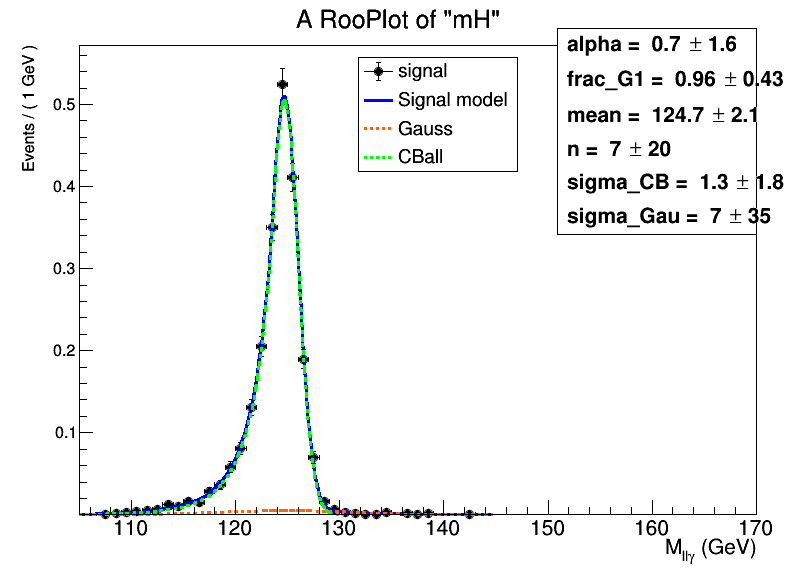
\includegraphics[width=0.40\textwidth]{fig/signal_fit/2016/sigfit_ele_ggF_2_125.png}\\
		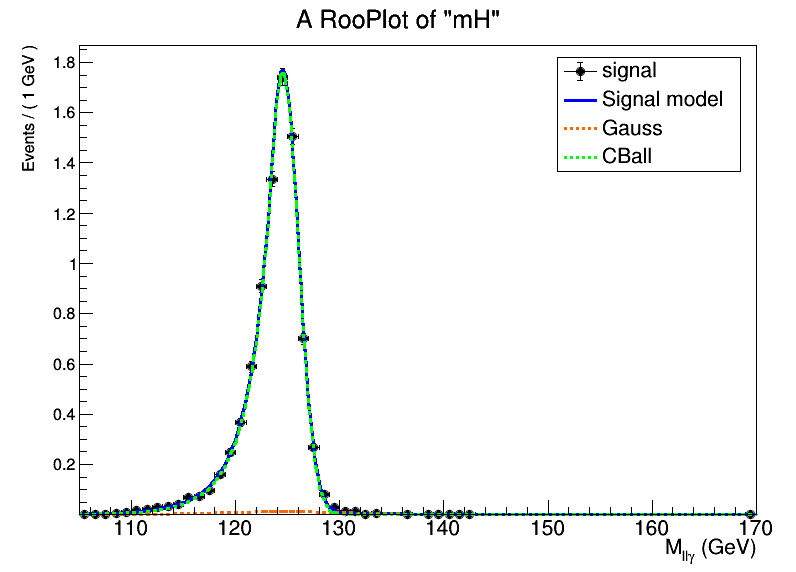
\includegraphics[width=0.40\textwidth]{fig/signal_fit/2016/sigfit_ele_ggF_3_125.png}
		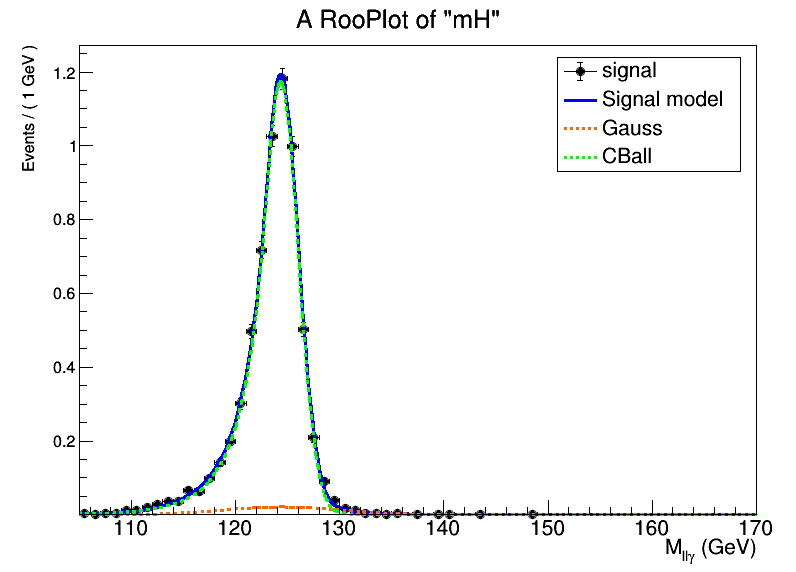
\includegraphics[width=0.40\textwidth]{fig/signal_fit/2016/sigfit_ele_ggF_4_125.png}\\
		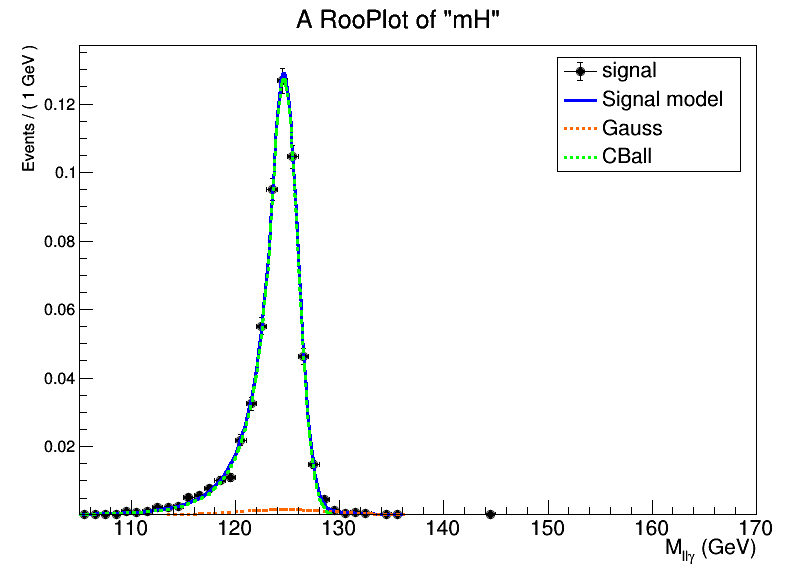
\includegraphics[width=0.40\textwidth]{fig/signal_fit/2016/sigfit_ele_VBF_501_125.png}
		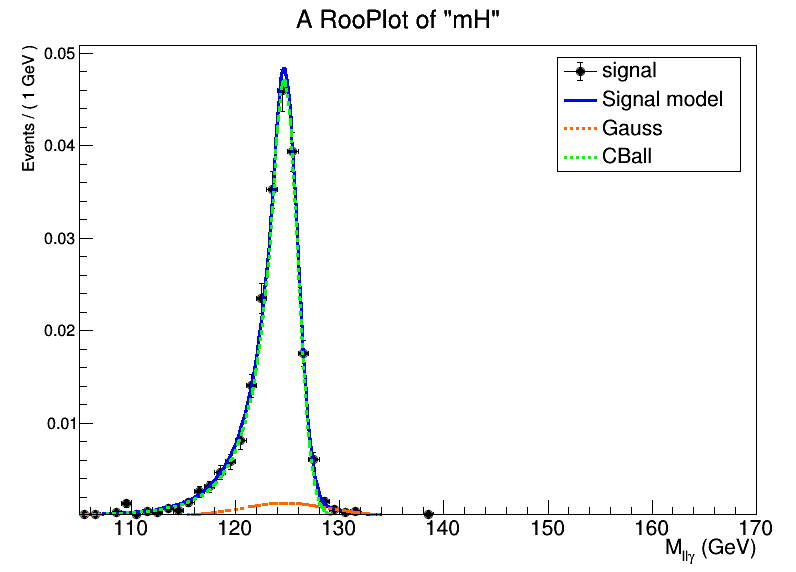
\includegraphics[width=0.40\textwidth]{fig/signal_fit/2016/sigfit_ele_VBF_502_125.png}\\
		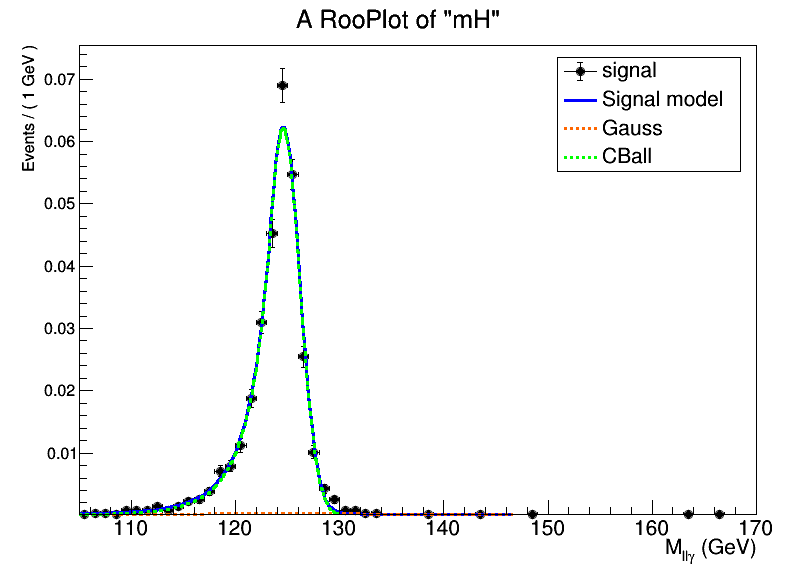
\includegraphics[width=0.40\textwidth]{fig/signal_fit/2016/sigfit_ele_VBF_503_125.png}\\
		\caption{Fits to simulated $m_{\ell^+\ell^-\gamma}$ signal distributions in the electron channel for
            		 $m_\PH=125\GeV$ for the 2016 data-taking period.
			 The blue line shows the total fit function, the green line shows the Crystal Ball function component, and the red line shows the Gaussian function component.
			 The top four plots correspond to the untagged categories, and the bottom three plots correspond to the dijet categories.}
		\label{fig:elesigfit}
	\end{center}
\end{figure}

\begin{figure}
	\begin{center}
		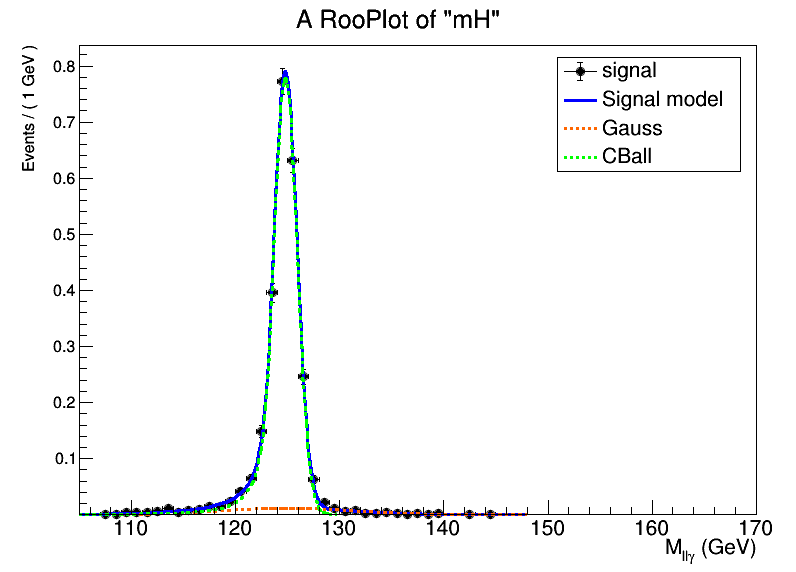
\includegraphics[width=0.40\textwidth]{fig/signal_fit/2016/sigfit_mu_ggF_1_125.png}
		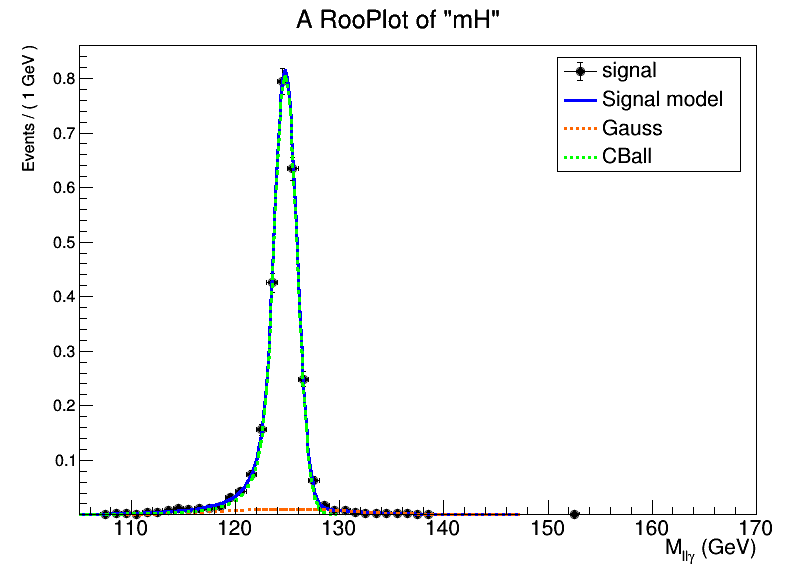
\includegraphics[width=0.40\textwidth]{fig/signal_fit/2016/sigfit_mu_ggF_2_125.png}\\
		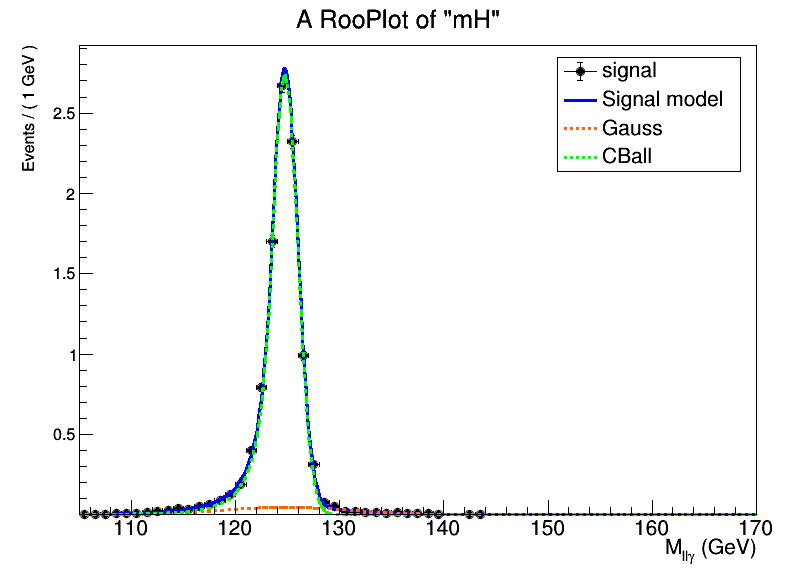
\includegraphics[width=0.40\textwidth]{fig/signal_fit/2016/sigfit_mu_ggF_3_125.png}
		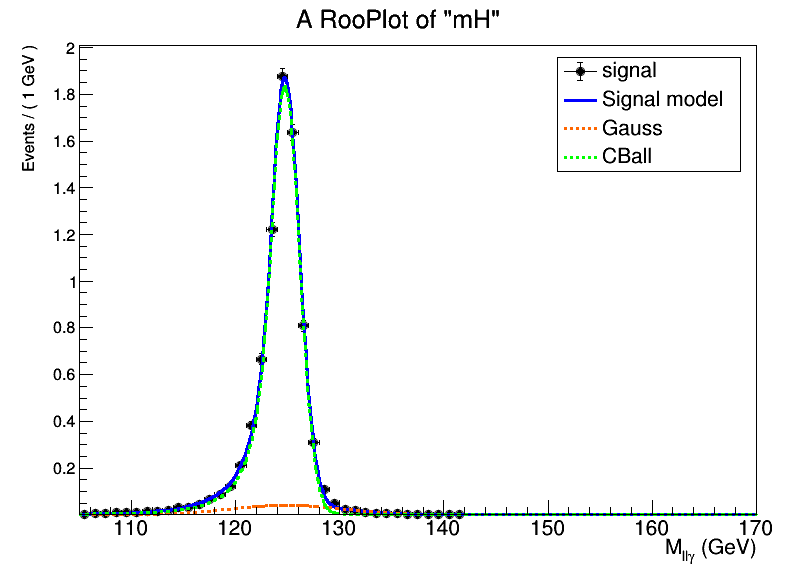
\includegraphics[width=0.40\textwidth]{fig/signal_fit/2016/sigfit_mu_ggF_4_125.png}\\
		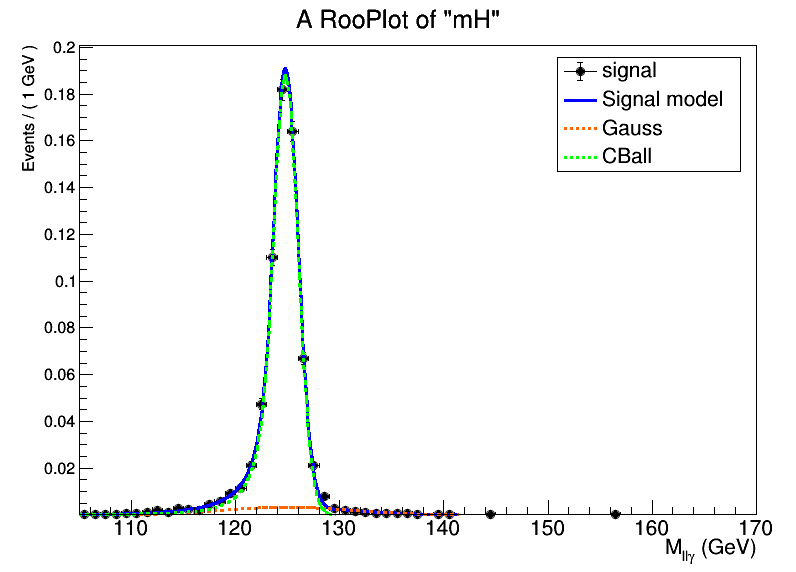
\includegraphics[width=0.40\textwidth]{fig/signal_fit/2016/sigfit_mu_VBF_501_125.png}
		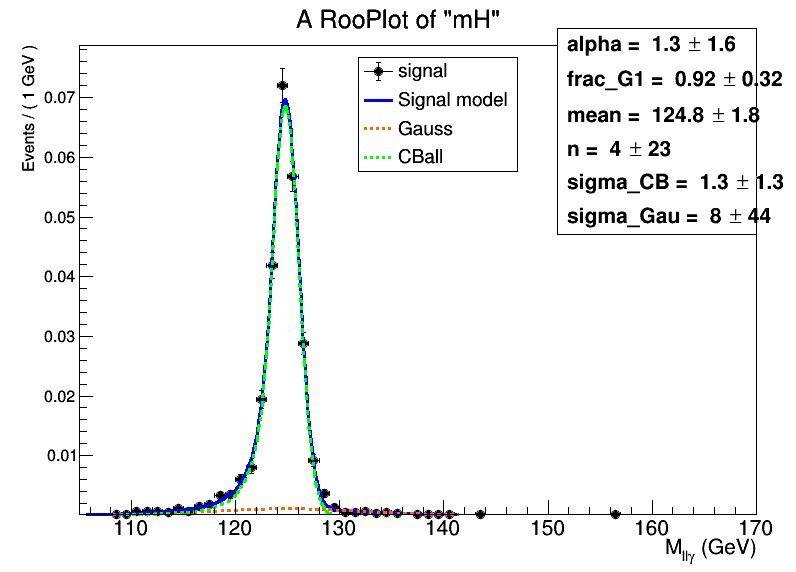
\includegraphics[width=0.40\textwidth]{fig/signal_fit/2016/sigfit_mu_VBF_502_125.png}\\
		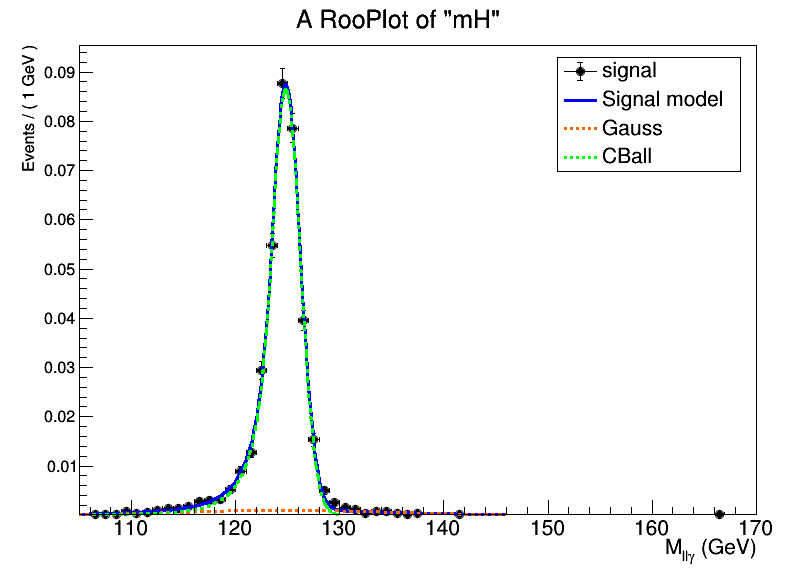
\includegraphics[width=0.40\textwidth]{fig/signal_fit/2016/sigfit_mu_VBF_503_125.png}\\
		\caption{Fits to simulated $m_{\ell^+\ell^-\gamma}$ signal distributions in the muon channel for
            		 $m_\PH=125\GeV$ for the 2016 data-taking period.
			 The blue line shows the total fit function, the green line shows the Crystal Ball function component, and the red line shows the Gaussian function component.
			 The top four plots correspond to the untagged categories, and the bottom three plots correspond to the dijet categories.}
		\label{fig:elesigfit}
	\end{center}
\end{figure}

\begin{figure}
	\begin{center}
	  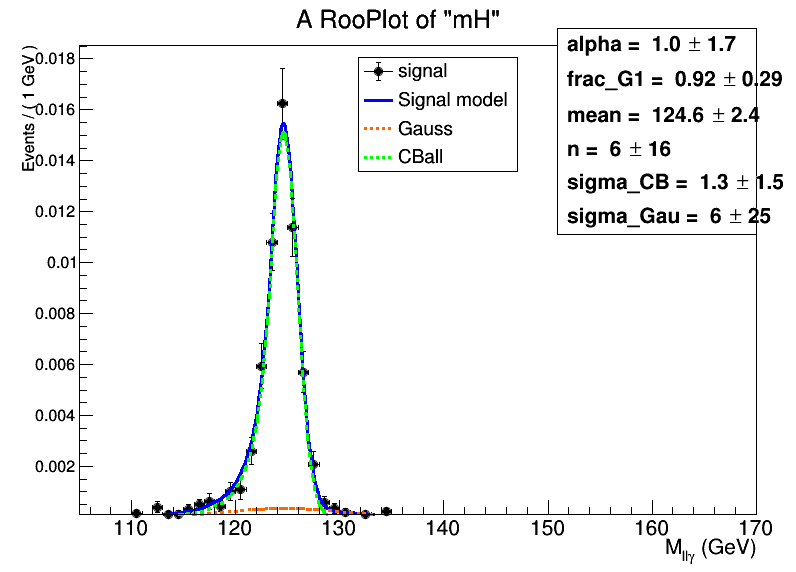
\includegraphics[width=0.40\textwidth]{fig/signal_fit/2016/sigfit_ele_mu_ZH_6789_125.png}
	  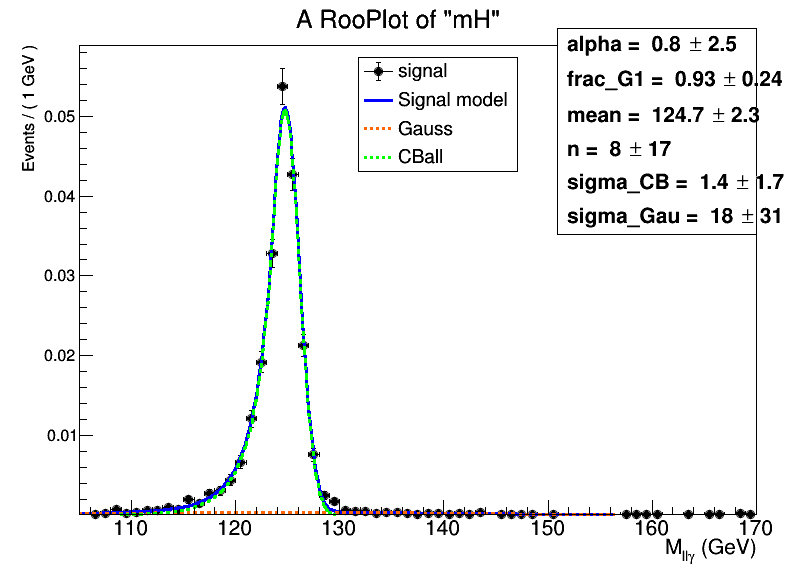
\includegraphics[width=0.40\textwidth]{fig/signal_fit/2016/sigfit_ele_mu_WH_6789_125.png}
		\caption{Fits to simulated $m_{\ell^+\ell^-\gamma}$ signal distributions in the electron and muon channels combined in the lepton-tagged category for
            		 $m_\PH=125\GeV$ for the 2016 data-taking period.
        		 The left plot shows the fit to simulated ZH production events, and the right plot shows the fit to simulated WH production events. 
			 The blue line shows the total fit function, the green line shows the Crystal Ball function component, and the red line shows the Gaussian function component.}
		\label{fig:elemusigfit}
	\end{center}
\end{figure}

\section{Resonant Background Modeling}

The process $\PH\to\Pgmp\Pgmm$, where at least one muon radiates an FSR photon, is expected to contribute at the 6\% level relative to the $\PH\to\PZ\PGg$ signal yield. Because of this, 
we treat it as a resonant background. To model the $\PH\to\Pgmp\Pgmm$ shape, we perform fits to the $m_{\ell^+\ell^-\gamma}$ distributions in simulated event samples, following the same 
procedure used for the signal fits described above. As for the signal, the analytic model is taken to be the sum of Crystal Ball and Gaussian functions. The resulting fits are shown 
in Figs. [REF]. 


\begin{figure}
	\begin{center}
		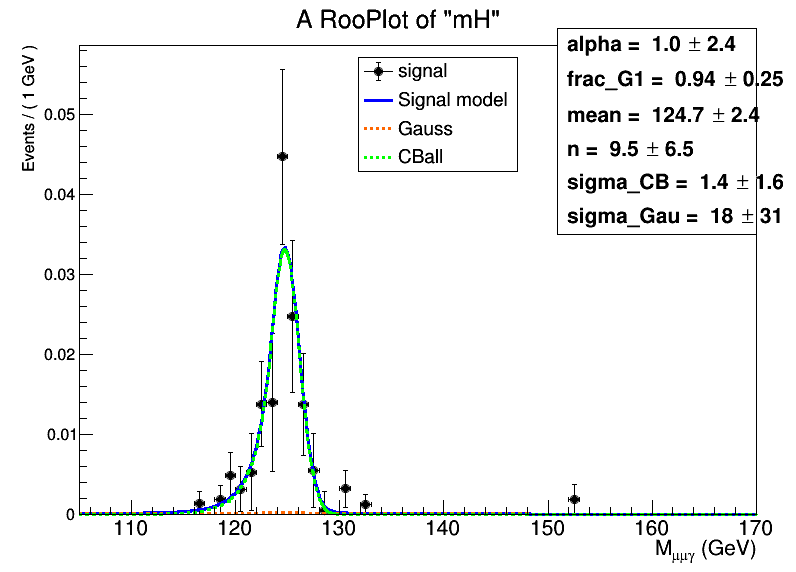
\includegraphics[width=0.40\textwidth]{fig/hmumu/2016/bkgfit_mu_ggF_1_125.png}
		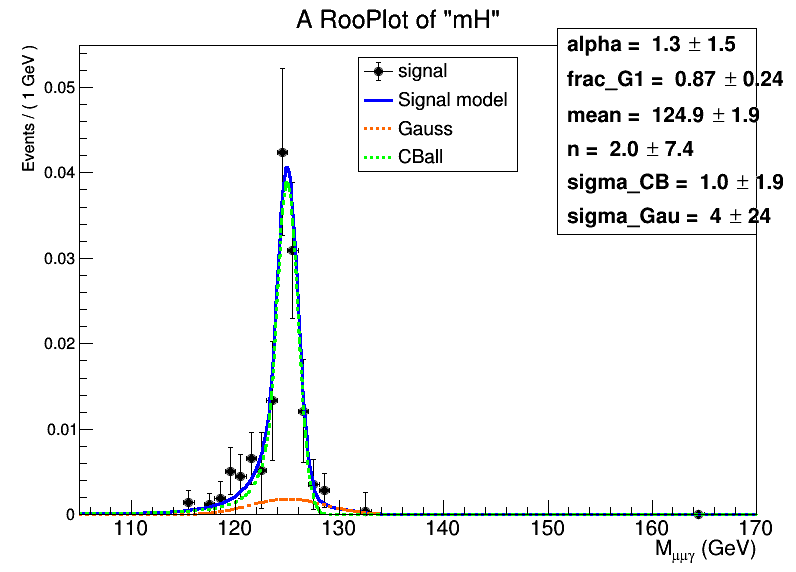
\includegraphics[width=0.40\textwidth]{fig/hmumu/2016/bkgfit_mu_ggF_2_125.png}\\
		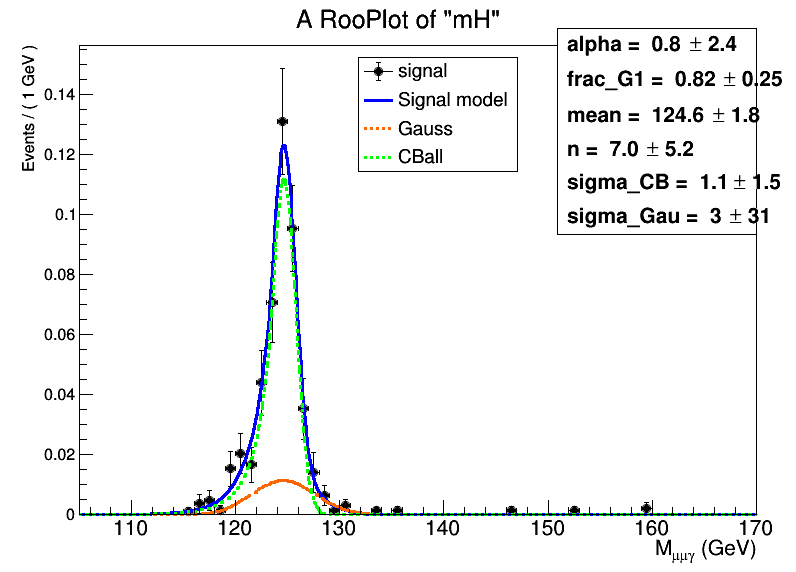
\includegraphics[width=0.40\textwidth]{fig/hmumu/2016/bkgfit_mu_ggF_3_125.png}
		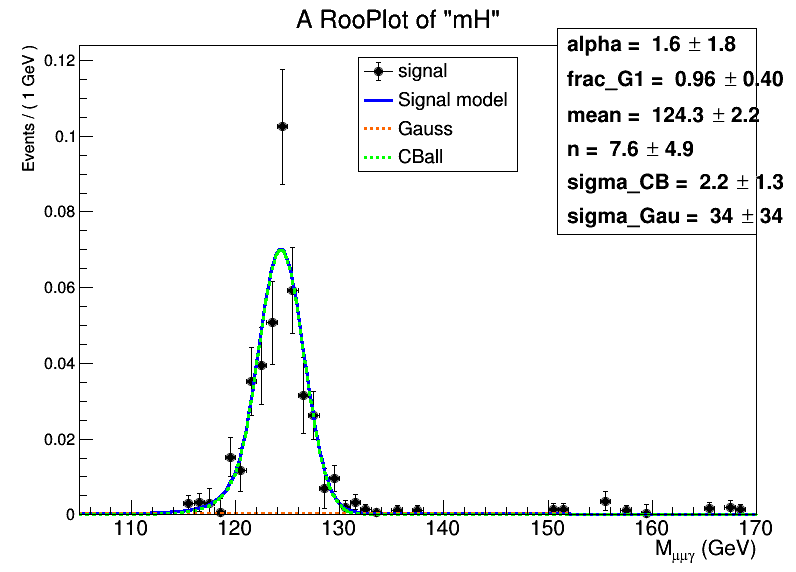
\includegraphics[width=0.40\textwidth]{fig/hmumu/2016/bkgfit_mu_ggF_4_125.png}\\
		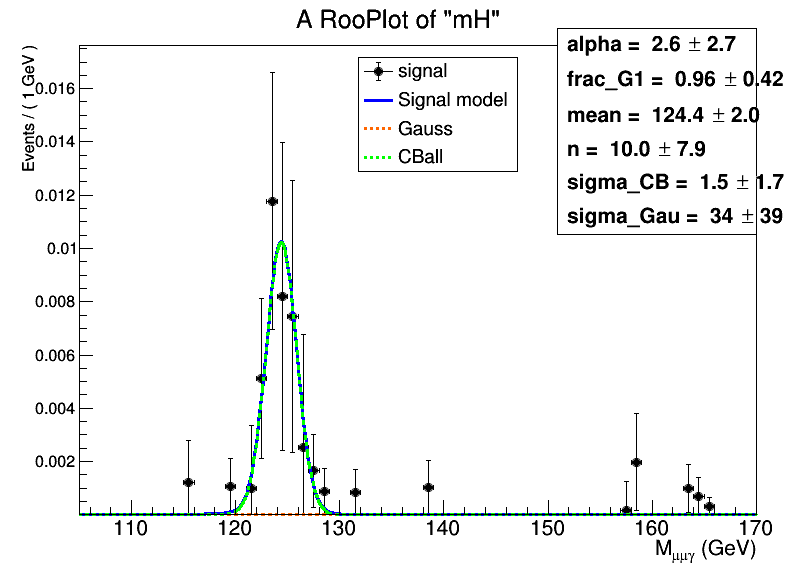
\includegraphics[width=0.40\textwidth]{fig/hmumu/2016/bkgfit_mu_VBF_501_125.png}
		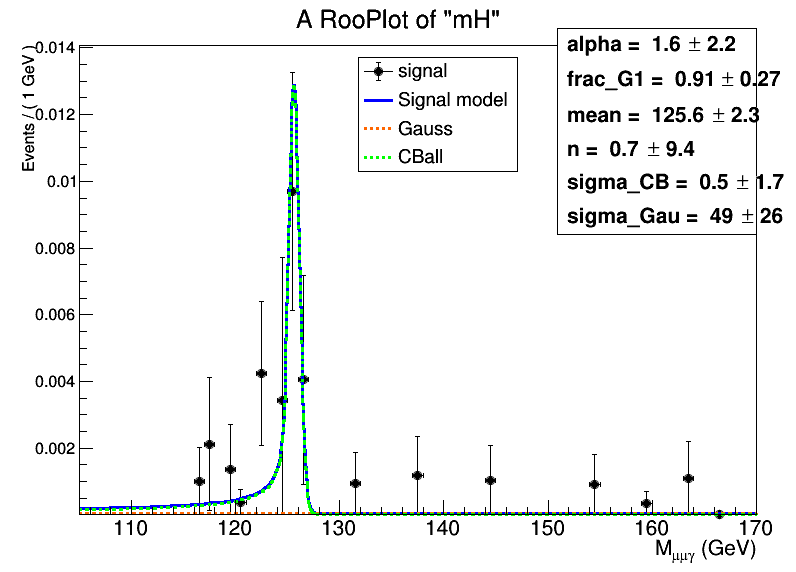
\includegraphics[width=0.40\textwidth]{fig/hmumu/2016/bkgfit_mu_VBF_502_125.png}\\
		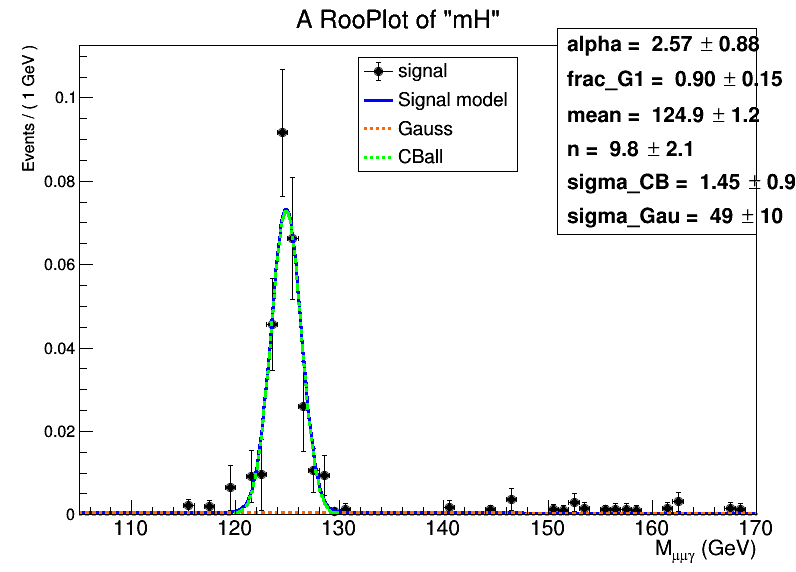
\includegraphics[width=0.40\textwidth]{fig/hmumu/2016/bkgfit_mu_ggF_503_125.png}
		\caption{Fits to simulated $m_{\mu^+\mu^-\gamma}$ resonant background distributions from $\PH\to\Pgmp\Pgmm$ for
			 $m_\PH=125\GeV$ for the 2016 data-taking period.
			 The blue line shows the total fit function, the green line shows the Crystal Ball function component, and the red line shows the Gaussian function component.
			 The top four plots correspond to the untagged categories, and the bottom three plots correspond to the dijet categories.}
		\label{fig:mubkgfit}
	\end{center}
\end{figure}

\begin{figure}
	\begin{center}
		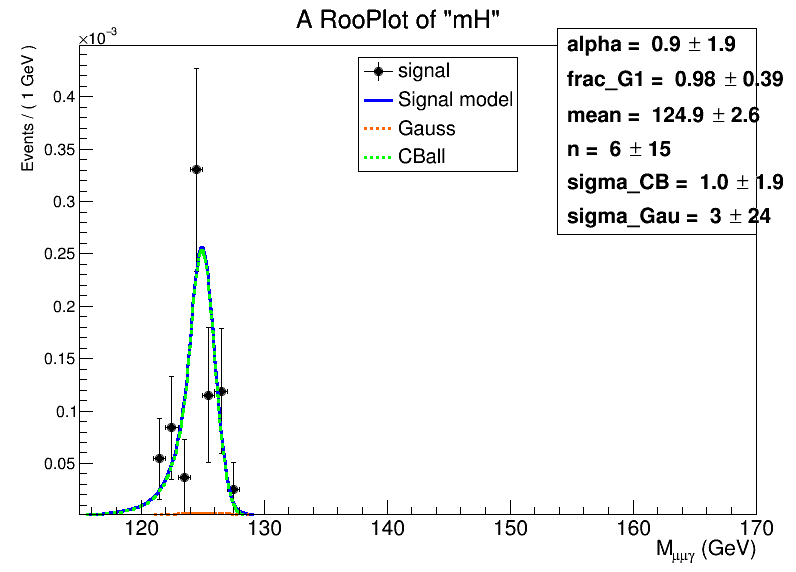
\includegraphics[width=0.40\textwidth]{fig/hmumu/2016/bkgfit_ele_mu_ZH_6789_125.png}
		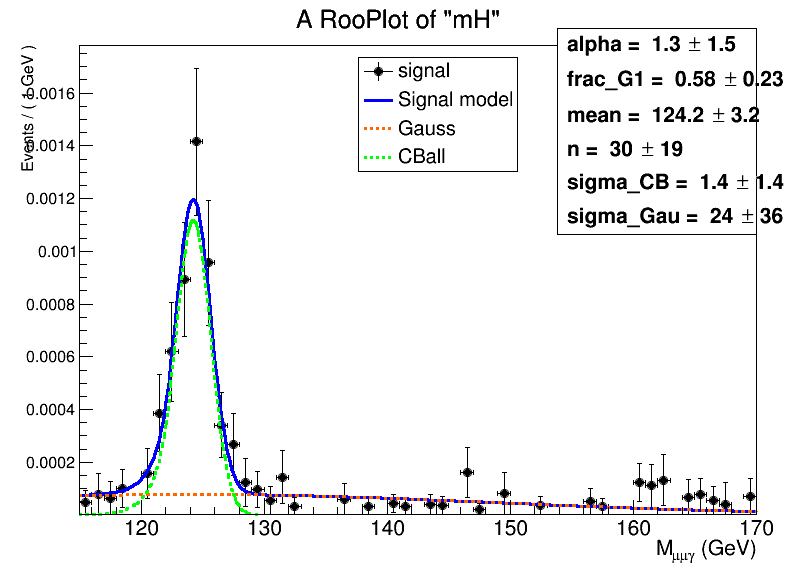
\includegraphics[width=0.40\textwidth]{fig/hmumu/2016/bkgfit_ele_mu_WH_6789_125.png}
		\caption{Fits to simulated $m_{\ell^+\ell^-\gamma}$ resonant background distributions from $\PH\to\Pgmp\Pgmm$ in the electron and muon channels combined in the lepton-tagged category for
            		 $m_\PH=125\GeV$ for the 2016 data-taking period.
        		 The left plot shows the fit to simulated ZH production events, and the right plot shows the fit to simulated WH production events. 
			 The blue line shows the total fit function, the green line shows the Crystal Ball function component, and the red line shows the Gaussian function component.}
		\label{fig:elemubkgfit}
	\end{center}
\end{figure}

\section{Nonresonant Background Modeling}
As in previous versions of the analysis, we use a parametric fit to the $m_{\ell^+\ell^-\gamma}$ spectrum in data to estimate the background. 
The background model in each category is obtained from the data using the discrete profiling method~\cite{Dauncey:2014xga}.
This technique accounts for the systematic uncertainty associated with choosing an analytic functional form to fit the background.
The background function is chosen from a set of candidate functions via a discrete nuisance parameter in the fit. 
These functions are derived from the data in each category, with muon and electron events from all data-taking years combined.
The discrete profiling method is described in further detail later in this section. 

In Run 1 \cite{CMS-PAS-HIG-13-006}, the background fitting started from 100\GeV. 
At the lower end of this fit range, below about 115 \GeV, there is a notable turn-on in the mass distribution that arises due to the 
presence of the on-shell Z boson. As such, the Run 1 analysis used PDFs composed of a Gaussian turn-on component convoluted 
with a falling spectrum component. In the first Run 2 analysis using only the 2016 data, this procedure was significantly changed.
The lower bound of the fit range was updated to 115 \GeV in order to avoid the turn-on. This meant that the functional forms used
to model the background could be simplified, as they no longer required the turn-on component. Now, in the full Run 2 analysis with 
2016, 2017, and 2018 data, we have returned to the Run 1 approach of fitting the turn-on. The reason for this is that the turn-on can have an impact on 
the mass distribution, even above 115 \GeV. As a consequence, avoiding the turn-on component of the fit leads to some mismodeling in the 
low mass region. Moreover, this mismodeling can be enough in some cases to lead to significant bias in the signal strength measurement. 
The solution has been to set the lower bound at 105 \GeV such that the turn-on is roughly Gaussian and can be modeled and fit properly.

\subsection{General Form of PDFs}
The $m_{\ell^+\ell^-\gamma}$ spectrum consists of a turn-on peak around 110--115\GeV and a falling spectrum in the high-mass tail, where the turn-on peak is driven by the photon $\pt$ selection. 
These features are modeled by the convolution of a Gaussian function with a step function multiplied by one of several falling spectrum functions.
The complete function has the general form:
% To model the background distribution, we consider functions with the following general form:
\begin{equation}
    \mathcal{F}(m_{\ell^+\ell^-\gamma}; \mu_{\mathrm{G}}, \sigma_{\mathrm{G}}, s, \vec{\alpha}) = \int_{105}^{170}\mathcal{N}(m_{\ell^+\ell^-\gamma}-t;\mu_{\mathrm{G}},\sigma_{\mathrm{G}})\Theta(t; s)f(t; \vec{\alpha})dt,
\end{equation}
where $t$ is the integration variable for the convolution, $\mathcal{N}(m_{\ell^+\ell^-\gamma}-t;\mu_{\mathrm{G}},\sigma_{\mathrm{G}})$ is the Gaussian function with mean $\mu_{\mathrm{G}}$ and standard deviation $\sigma_{\mathrm{G}}$, $\Theta(t; s)$ is the Heaviside step function with step location $s$, and $f(t; \vec{\alpha})$ is the falling spectrum function with shape parameters $\vec{\alpha}$.
The total number of parameters in the fit is equal to three plus the number of parameters 
in the falling spectrum component.

\subsection{Falling Spectrum Component Families}
The choice of falling spectrum component to model the background in a given category is not a priori known. For this reason, we consider several 
families of PDFs for the falling spectrum. The families tested include Bernstein polynomials, exponential series, power law series, and 
Laurent series. These families are described in more detail as follows:

\begin{itemize}
	\item exponential series of order N:
	\begin{equation}
        \mathrm{Exp_{N}}(m_{\ell\ell\gamma}) = \sum\limits_{i=1}^{N}f_ie^{p_i\, m_{\ell\ell\gamma}}
	\end{equation}
	with $2N$ free parameters: $p_i < 0$ and $f_i$.
	The lowest order considered has $N=1$, i.e. one term.
	The next order has 2 exponential terms, but 3 parameters.	

	\item power law series of order N:
	\begin{equation}
        \mathrm{Pow_{N}}(m_{\ell\ell\gamma}) = \sum\limits_{i=1}^{N}f_im_{\ell\ell\gamma}^{p_i}
	\end{equation}
	with $2N$ free parameters: $p_i < 0$ and $f_i$.
	The lowest order considered has $N=1$, i.e. one term.
	
	\item Bernstein polynomial of order N:
    \begin{equation}
        \mathrm{Bern_{N}}(m_{\ell\ell\gamma}) = \sum\limits_{i=0}^{N}f_{i}b_{i,N}(m_{\ell\ell\gamma})
    \end{equation}
    \begin{equation}
        \mathrm{b_{i,N}}(m_{\ell\ell\gamma}) = \binom{N}{i}m_{\ell\ell\gamma}^{i}(1 - m_{\ell\ell\gamma}^{N-i})
    \end{equation}
    with $N$ free parameters $f_{i}$. The lowest order considered has $N=1$.

	\item Laurent series with 2, 3, 4, 5, or 6 terms, where N + 1 equals the number of free parameters:
	\begin{equation}
        \mathrm{Lau_{1}}(m_{\ell\ell\gamma}) = f_2m_{\ell\ell\gamma}^{-4}+f_3m_{\ell\ell\gamma}^{-5}
	\end{equation}
	\begin{equation}
        \mathrm{Lau_{2}}(m_{\ell\ell\gamma}) = f_1m_{\ell\ell\gamma}^{-3}+f_2m_{\ell\ell\gamma}^{-4}+f_3m_{\ell\ell\gamma}^{-5}
	\end{equation}
	\begin{equation}
        \mathrm{Lau_{3}}(m_{\ell\ell\gamma}) = f_1m_{\ell\ell\gamma}^{-3}+f_2m_{\ell\ell\gamma}^{-4}+f_3m_{\ell\ell\gamma}^{-5}+f_4m_{\ell\ell\gamma}^{-6}
	\end{equation}
	\begin{equation}
        \mathrm{Lau_{4}}(m_{\ell\ell\gamma}) = f_1m_{\ell\ell\gamma}^{-2}+f_2m_{\ell\ell\gamma}^{-3}+f_3m_{\ell\ell\gamma}^{-4}+f_4m_{\ell\ell\gamma}^{-5}+f_5m_{\ell\ell\gamma}^{-6}
	\end{equation}
	\begin{equation}
        \mathrm{Lau_{5}}(m_{\ell\ell\gamma}) = f_1m_{\ell\ell\gamma}^{-2}+f_2m_{\ell\ell\gamma}^{-3}+f_3m_{\ell\ell\gamma}^{-4}+f_4m_{\ell\ell\gamma}^{-5}+f_5m_{\ell\ell\gamma}^{-6}+f_6m_{\ell\ell\gamma}^{-7}
	\end{equation}
\end{itemize}

\subsection{Discrete Profiling Method}\label{sec:envelope}
In each category, there is ambiguity about which PDF to choose to model the background. 
In previous versions of this analysis, a detailed bias study 
was performed for each falling spectrum component family, and the family with the least bias was chosen. However, 
no uncertainty was assigned due to the choice of background PDF. In principle, the 
choice of PDF is a source of systematic uncertainty in the measurement. 
Therefore, the discrete profiling method was since developed as a way to assess this uncertainty in a formal way. 
In this method, the choice of PDF for the background fit is included as a 
discrete nuisance parameter in the full likelihood function. All reasonable families of 
functions should be considered, and additionally, it is found that certain orders within 
the same family should be considered. The set of functions profiled in a given category is referred to as an \textit{envelope}.
The exact composition of the envelope in each category
is based on a set of selection requirements that account for goodness of fit, an F-test procedure, 
and an assessment of bias. The details of this selection will be described in the following section.
When fitting the background, all functions in the envelope are tried, with a penalty term added to the likelihood 
to account for the number of free parameters in the fit. When a measurement is made of 
a parameter of interest, for example the signal strength, the PDF with the smallest negative log likelihood, 
profiled as a function of the parameter of interest, is used. The profiling allows the best fit function to change for 
different values of the parameter of interest, so we can say that we carry out the fit with the full envelope of functions.  
The envelope yields a profile likelihood curve that is broader than the profile likelihood curve obtained from any individual function. 
This increase in breadth reflects the uncertainty associated with the choice of background PDF. 

\subsection{Envelope Selection}\label{sec:envelope_selection}
Individual functions are added to the envelope in a given category based on a series of selection requirements. In general, 
the requirements are related to three main factors: goodness of fit, F-test, and bias. The simplest requirement is a basic 
goodness of fit cut. For each function considered, the chi-squared per number of degrees of freedom is calculated. This is 
then converted into a p-value, or chi-squared probability. If the chi-squared probability is greater than 0.01, we consider 
the quality of the fit good enough for the envelope. Any function failing this requirement is thrown away, as it cannot
be considered a reasonable description of the data. 

The second consideration is the result of an F-test. The F-test is a way to compare functions within a specific family of 
falling spectrum component PDFs. It compares the fit of a lower order function in the family to that of a higher order function. 
While it is expected that the higher order function will always provide a better fit, the question is whether the higher order 
fit is better in a statistically significant way. If it is not significantly better, there is a motivation to stick to the lower
order function and exclude the higher order function from the envelope. The details of the F-test procedure are as follows. 
First, the lowest order PDF in a given family is fit to the data in a given
category. Then, the next highest order PDF is fit to the same data. The difference between twice 
the negative log likelihood between the two fits, $2\Delta NLL_{N+1} = 2(NLL_{N}-NLL_{N+1})$, 
can be used to determine whether the data are better supported by the higher order PDF. 
More precisely, $2\Delta NLL_{N+1}$ is distributed as a $\chi^{2}$ PDF with $M$ degrees of 
freedom, where $M$ is the difference in the number of free parameters between the order $N+1$ 
PDF and the order $N$ PDF. For example, in the case of the first two orders of 
the exponential family, $M = 4-2 = 2$, and for the Bernstein polynomial family, $M=3-2=1$. 
After carrying out the fits and computing the negative log likelihoods, a p-value is then 
calculated as 
\begin{equation}
\mathrm{p} = P(2\Delta NLL > 2\Delta NLL_{N+1} | \chi^{2}(M)).
\end{equation}
If the p-value is less than 0.05, we state that the higher order PDF is supported by the 
data, and the procedure is repeated for the next highest order PDF. Alternatively, if the 
p-value is greater than 0.05, the higher order PDF is assumed to be too flexible given 
the data, and the F-test ends, having found the highest order PDF supported by the data.
This procedure is done to find the highest-order PDF supported by the data for each PDF 
family. In this analysis, we consider fits up to order 5 for each falling spectrum family.
In each family, we identify the highest order function with an F-test probability below 0.05 and include it in the envelope. 
We then also include all lower order functions within the family that pass the chi-squared goodness of fit criterion.

The final consideration in selecting functions for the envelope is bias and coverage. After constructing an initial envelope in a given 
category based on the chi-squared and F-test results, an envelope bias study is performed. The full details of the envelope 
bias studies for each category can be reviewed in Section \ref{sec:envelope_bias_studies}. In a nutshell, toys are generated from 
each PDF contained in the envelope, and these toys are subsequently fit with the full envelope. The collection of toy fits
allows us to compute the bias and coverage of the signal strength. Should the bias and coverage be at an acceptable level, the 
envelope can be used in the analysis. However, in the presence of large bias or low coverage, we can consider modifying the 
composition of the envelope in order to reduce the bias. In practice, this is often achievable by adding higher order functions that 
may have been excluded by the F-test, but nevertheless fit the data well. These more flexible functions are often able to reduce the 
bias and improve the coverage of the envelope. This is considered category by category.
The fits of the chosen envelope functions in each category are shown in Figure \ref{fig:bkgmodel_e}.

\begin{figure}
	\begin{center}
        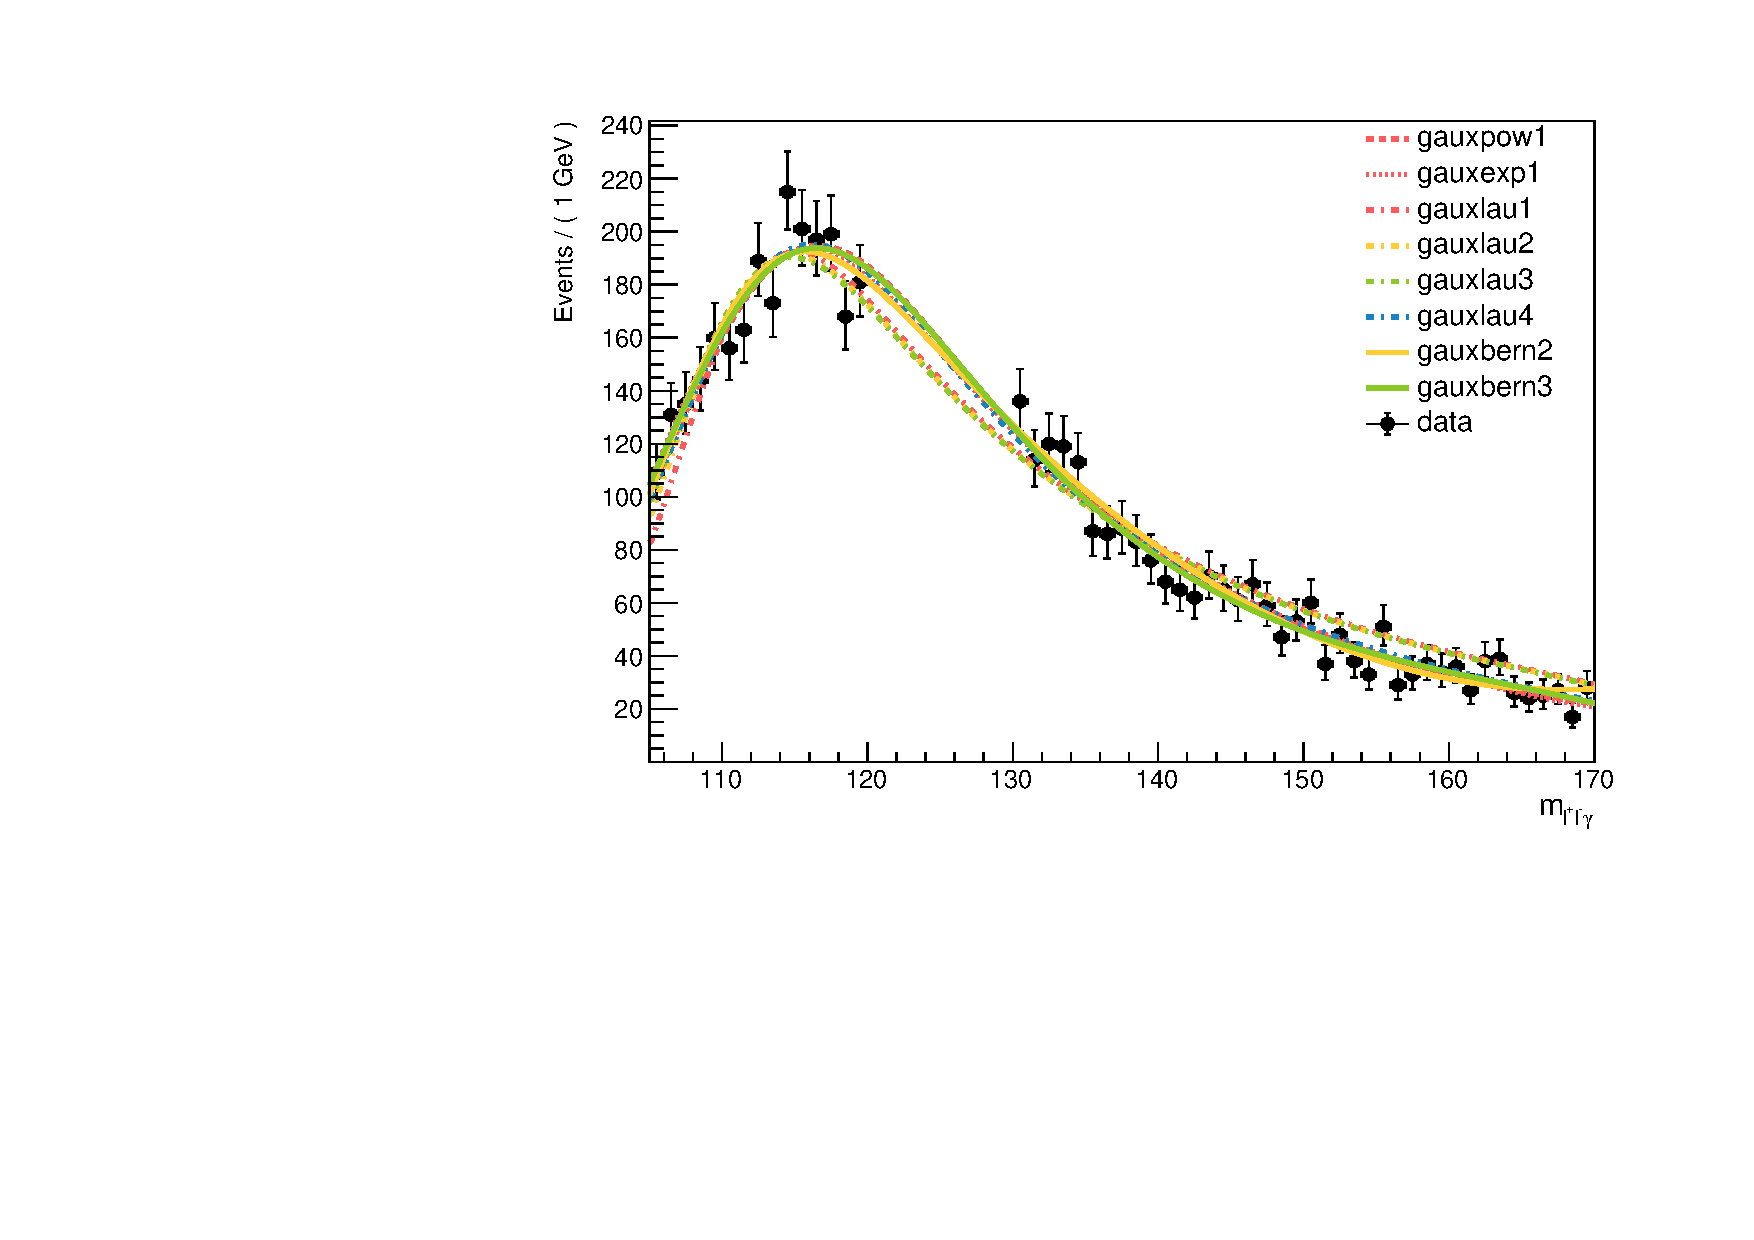
\includegraphics[width=0.4\textwidth]{fig/envelope_plots/m105_170_cat1_turn_lau.pdf}
        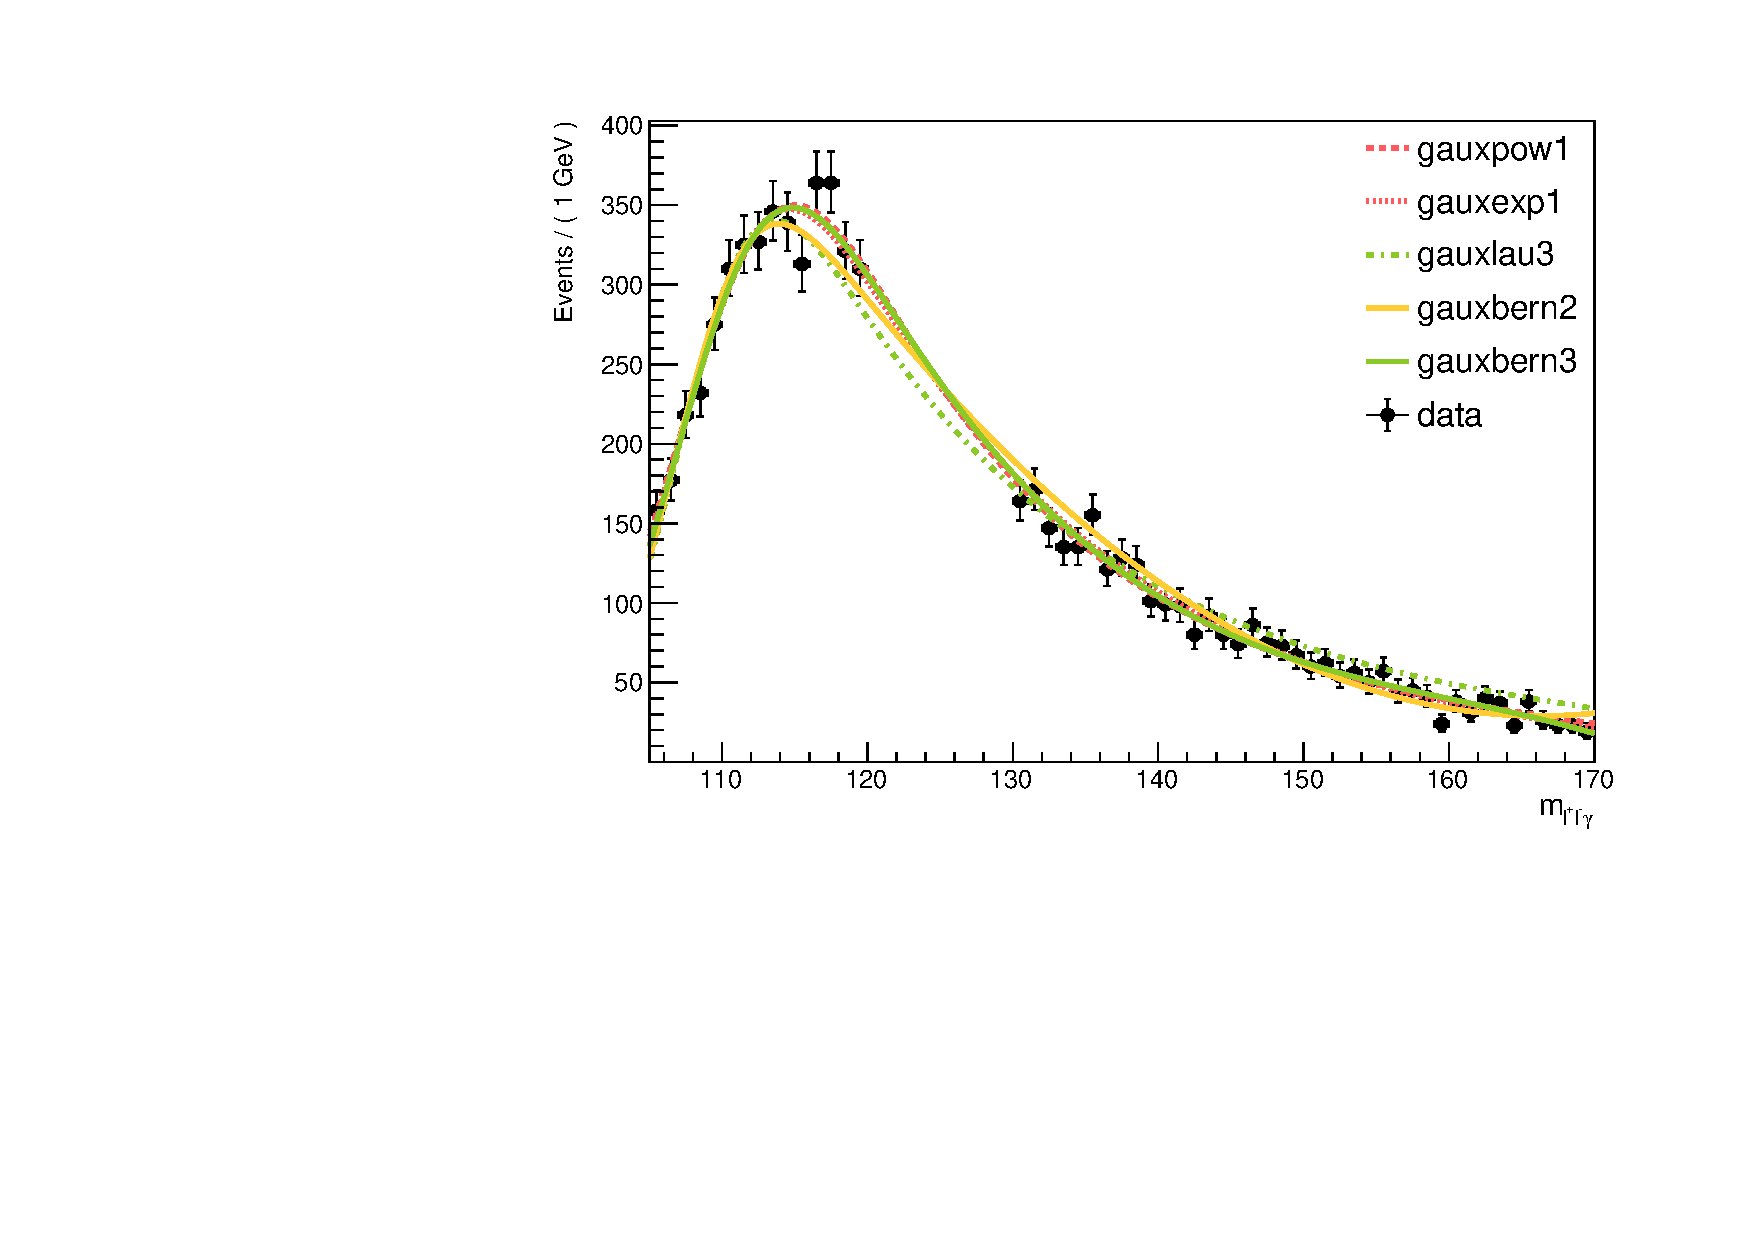
\includegraphics[width=0.4\textwidth]{fig/envelope_plots/m105_170_cat2_turn_lau.pdf}\\
        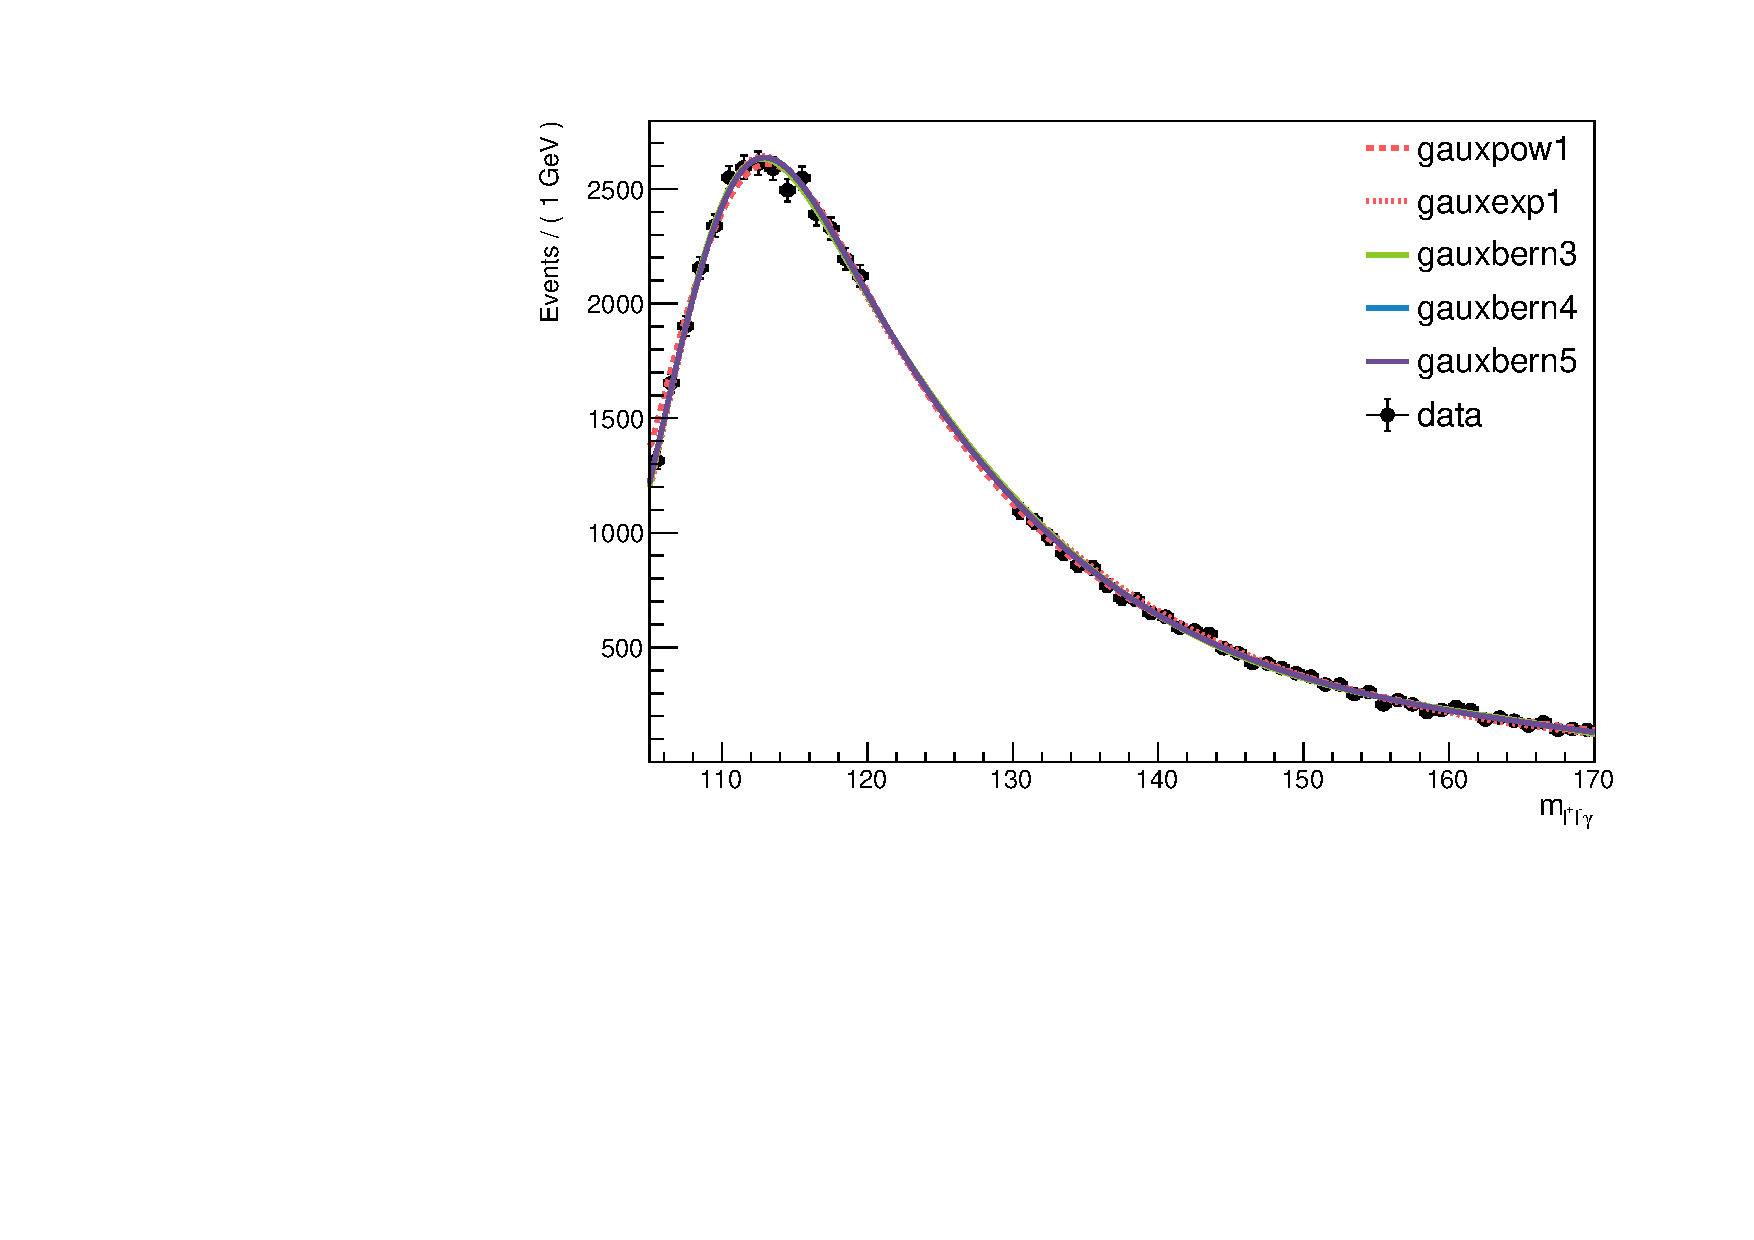
\includegraphics[width=0.4\textwidth]{fig/envelope_plots/m105_170_cat3_turn_bern5.pdf}
        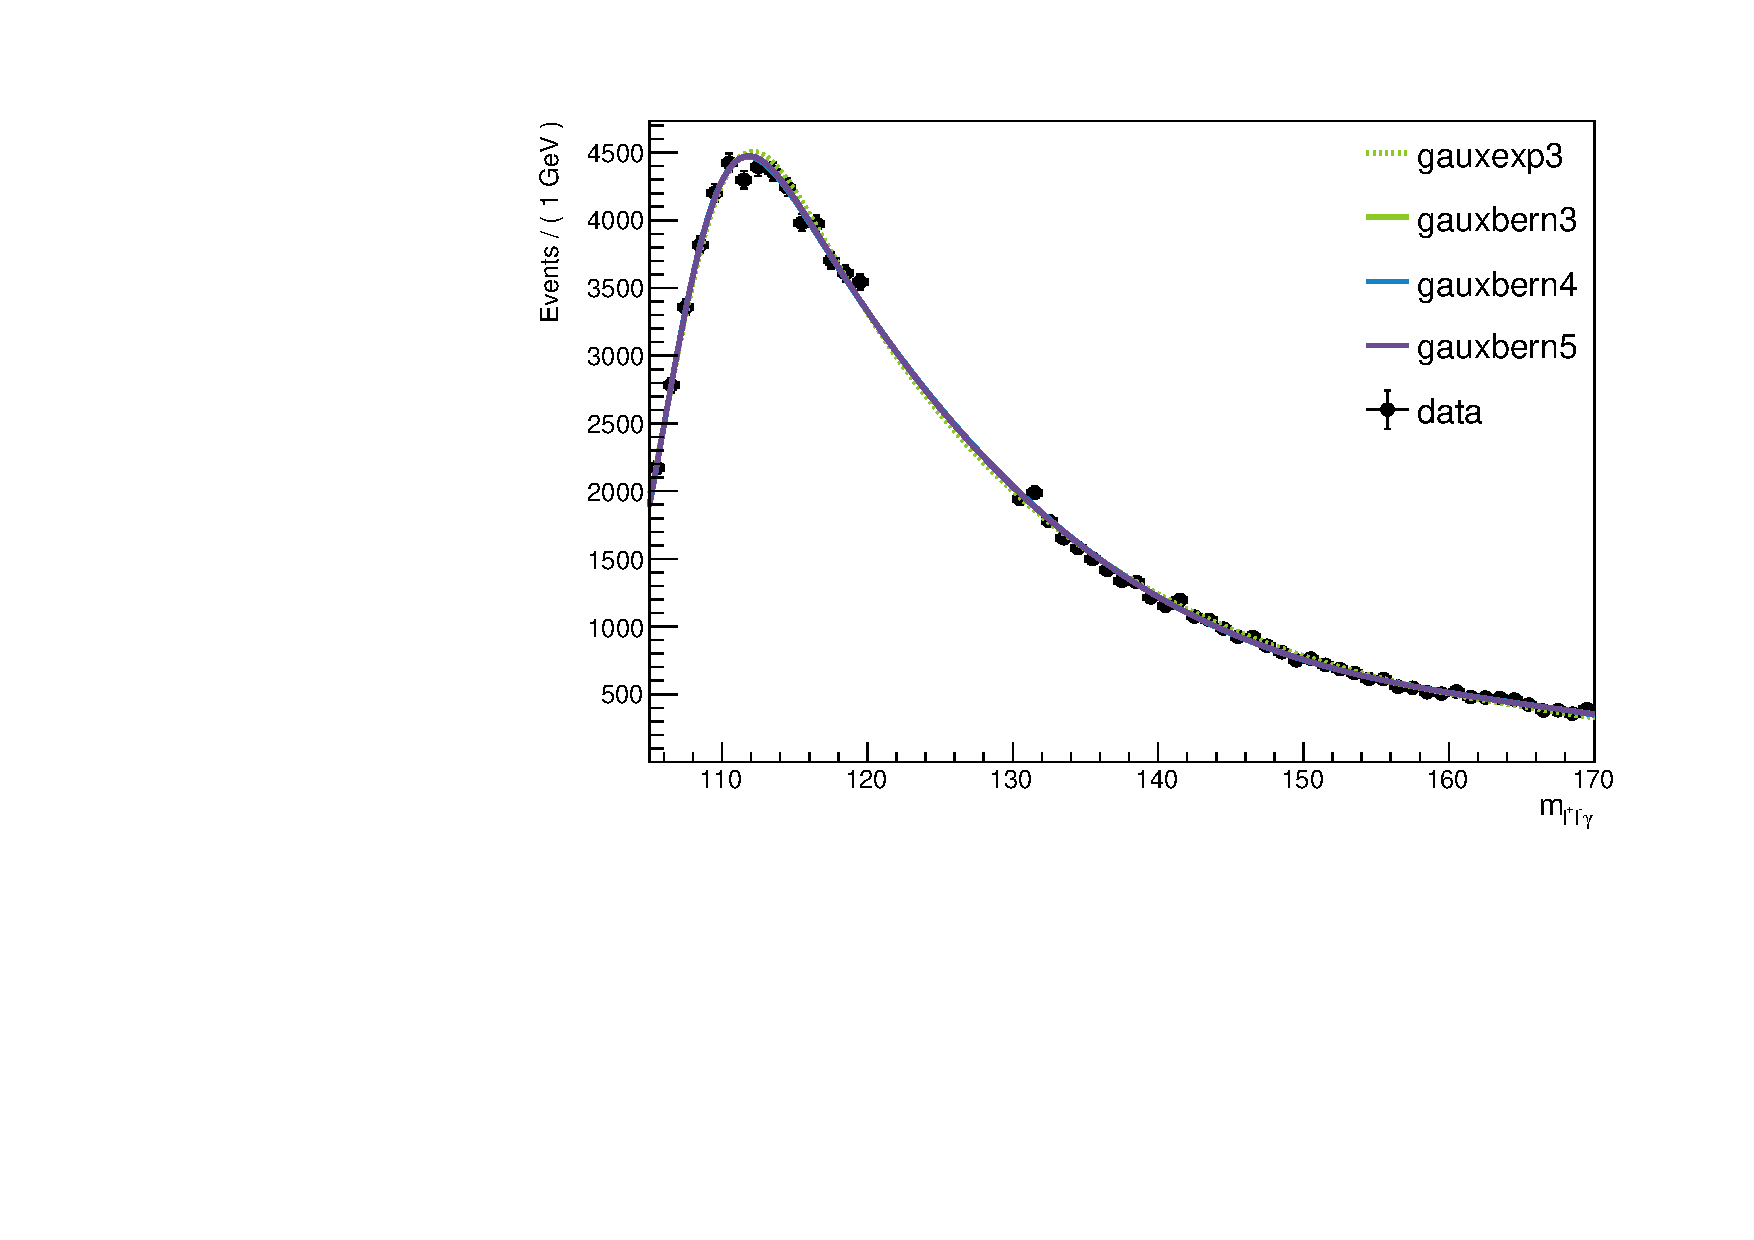
\includegraphics[width=0.4\textwidth]{fig/envelope_plots/m105_170_cat4_turn_bern5.pdf}\\
        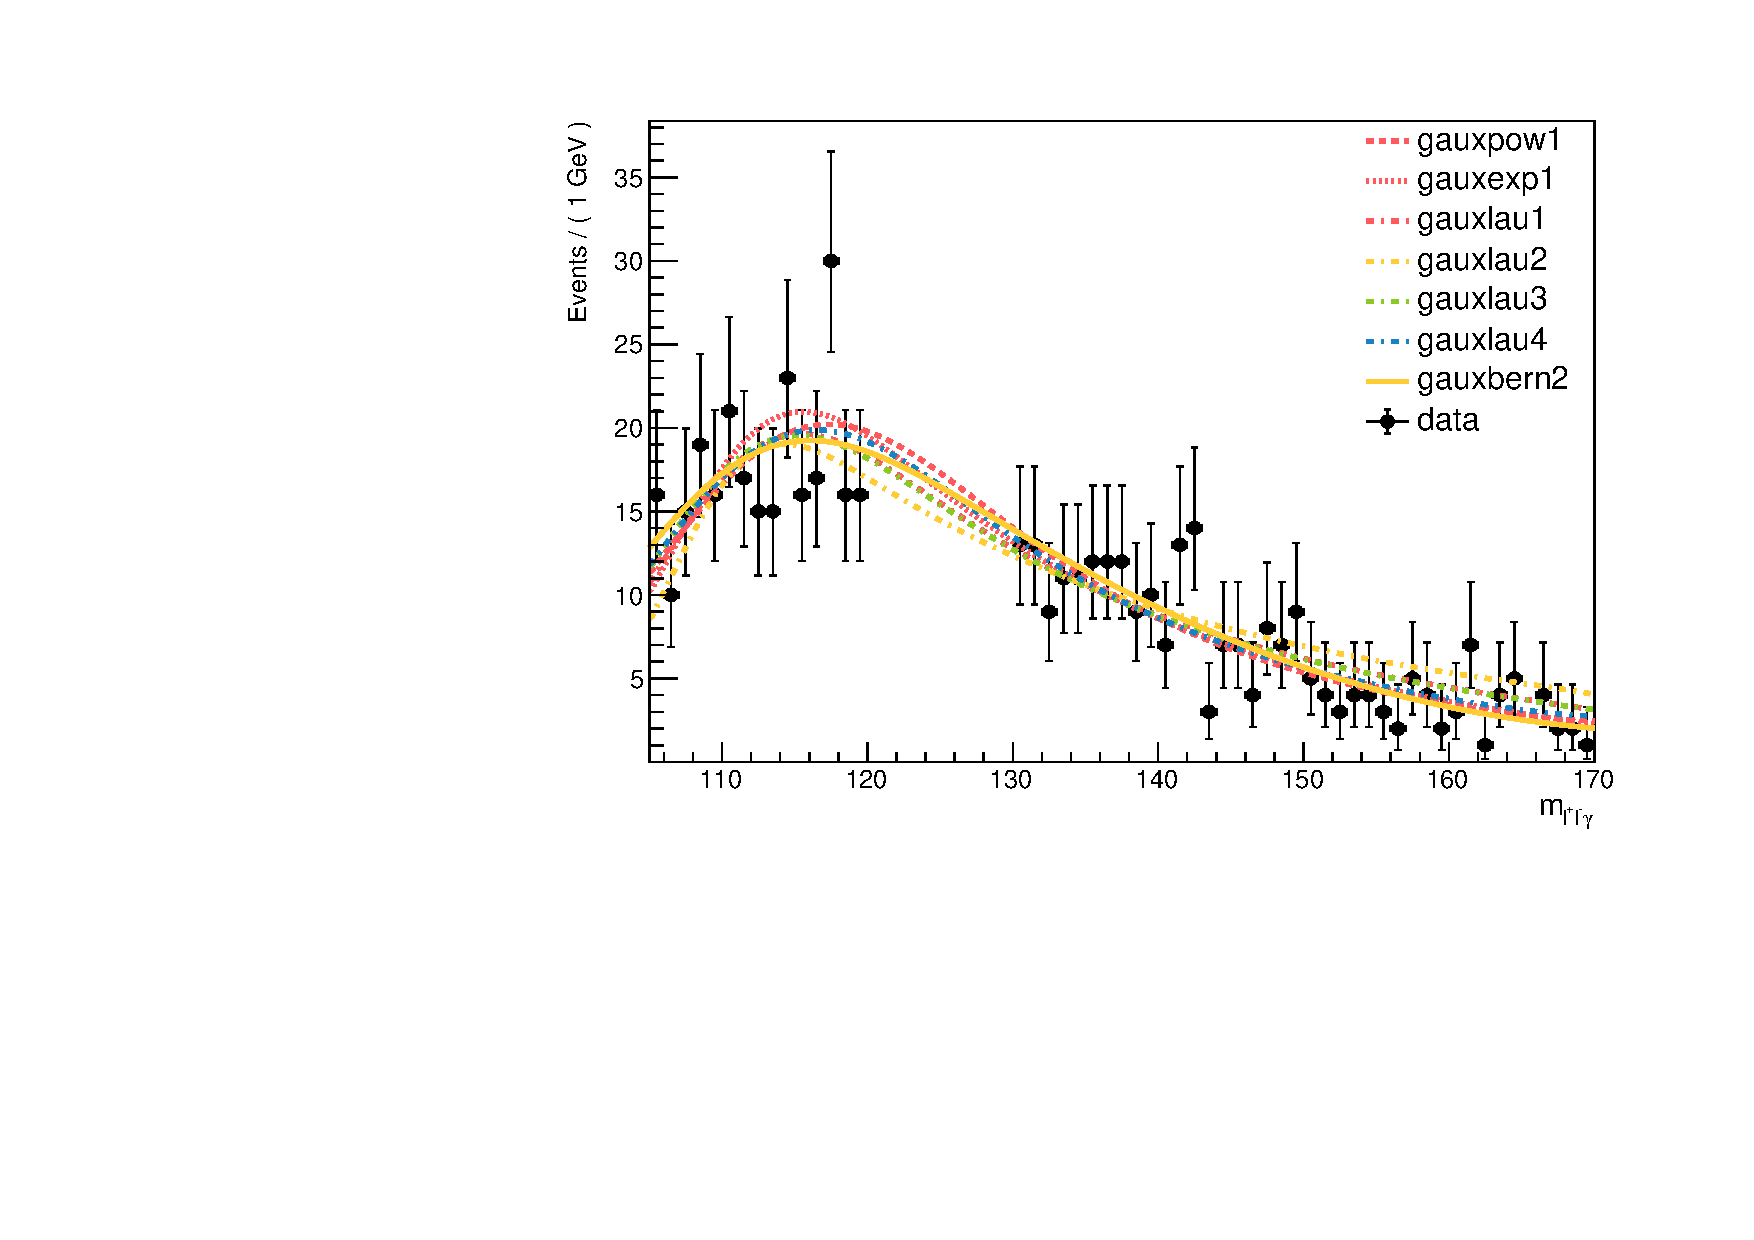
\includegraphics[width=0.4\textwidth]{fig/envelope_plots/m105_170_cat501_turn_lau.pdf}
        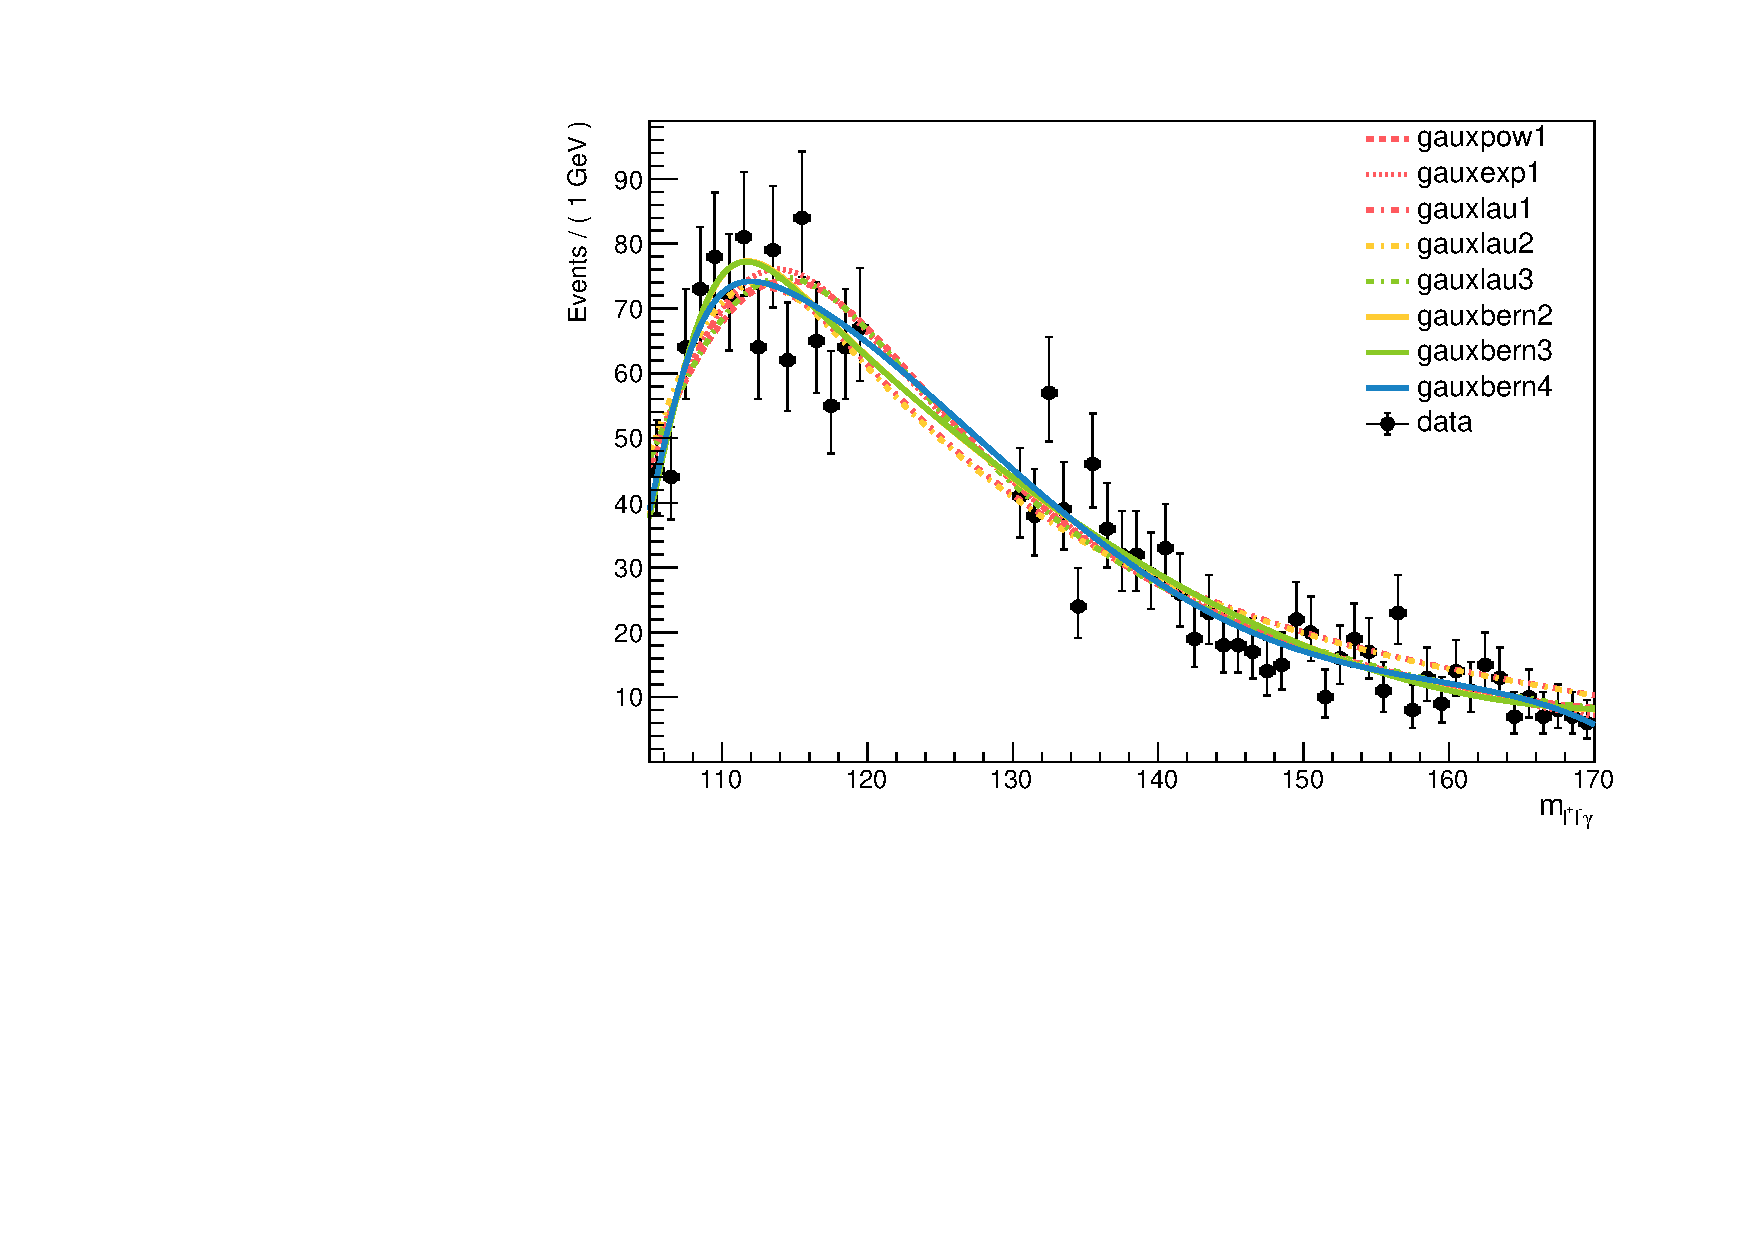
\includegraphics[width=0.4\textwidth]{fig/envelope_plots/m105_170_cat502_turn_lau.pdf}\\
        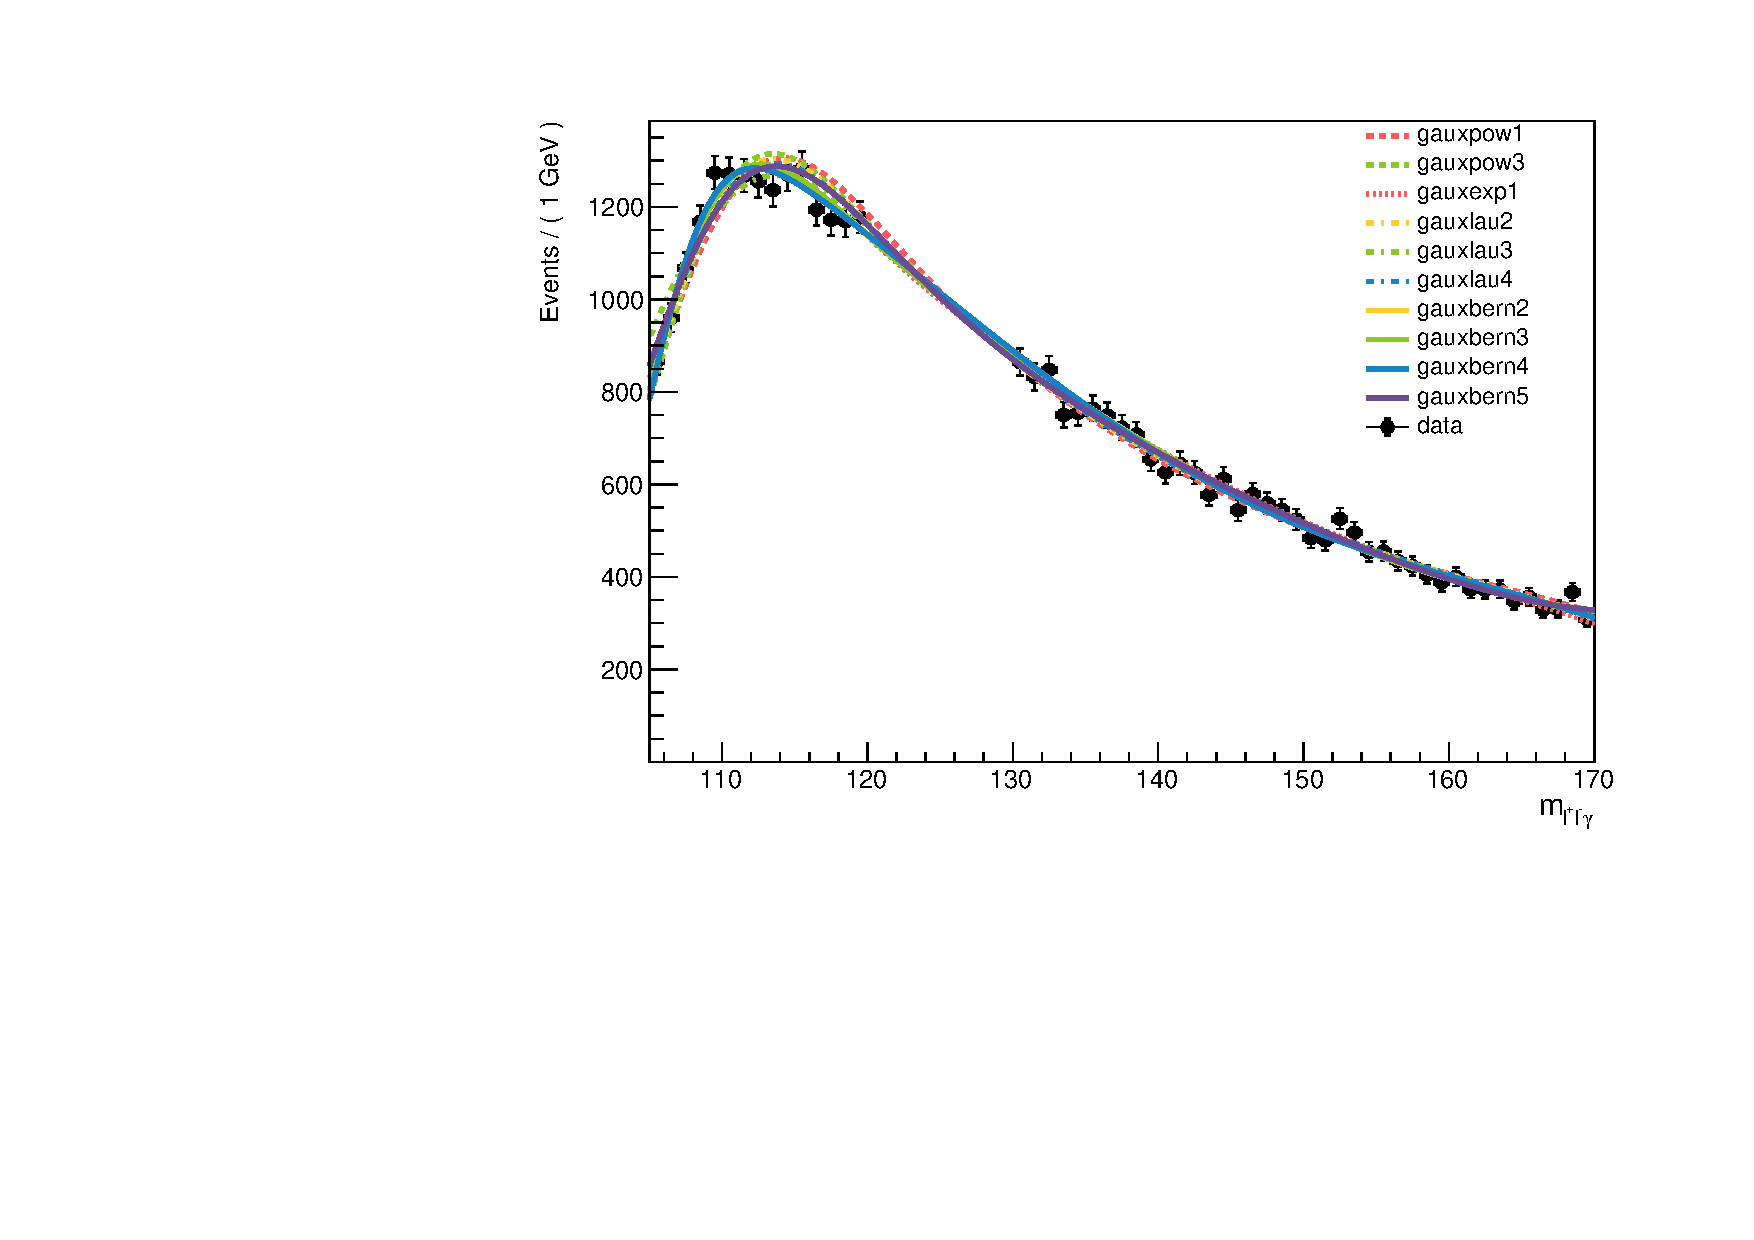
\includegraphics[width=0.4\textwidth]{fig/envelope_plots/m105_170_cat503_turn_bern5.pdf}
        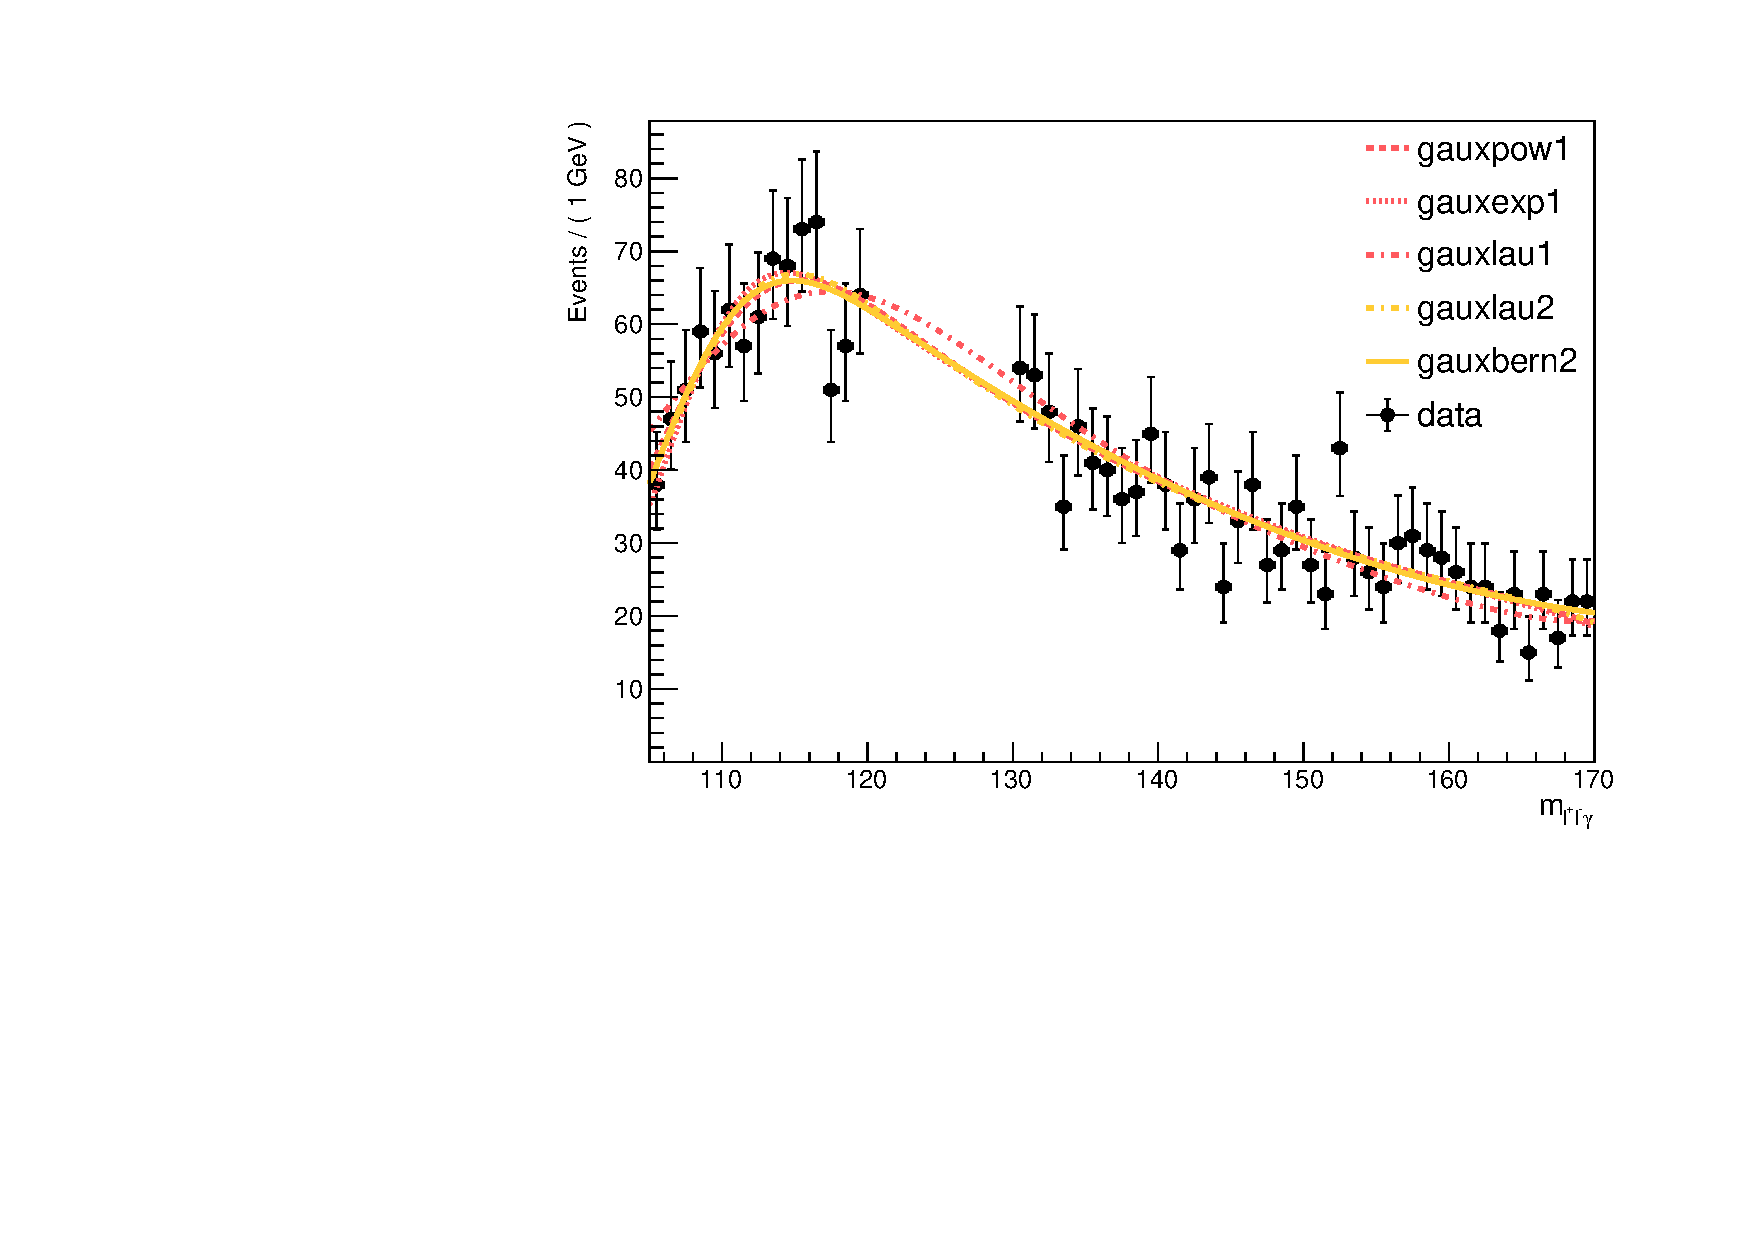
\includegraphics[width=0.4\textwidth]{fig/envelope_plots/m105_170_cat6789_turn_lau.pdf}
		\caption{Background functions determined by the discrete profiling method.
        The top four plots correspond to the untagged categories, and the bottom four plots correspond to the dijet categories and lepton tag category.}
		\label{fig:bkgmodel_e}
	\end{center}
\end{figure}

\subsection{Comparison with Previous Approach}
Previously, in the 2016 analysis and in earlier versions of the full Run 2 analysis, 
the background was modeled on the three body mass range 115 to 170 GeV. After extending the 
range down to 105 GeV and studying the fits in each category, it is worth checking how the new
modeling compares to the old. One simple way to compare is by overlaying the fit plots using 
the best fit function in each range. This is shown in Figure \ref{fig:compare_turnon_fits}. From the plots, 
it is clear that modeling the turn-on properly yields a better fit around 115 GeV, the previous lower bound of the fit. 

\begin{figure}
	\begin{center}
        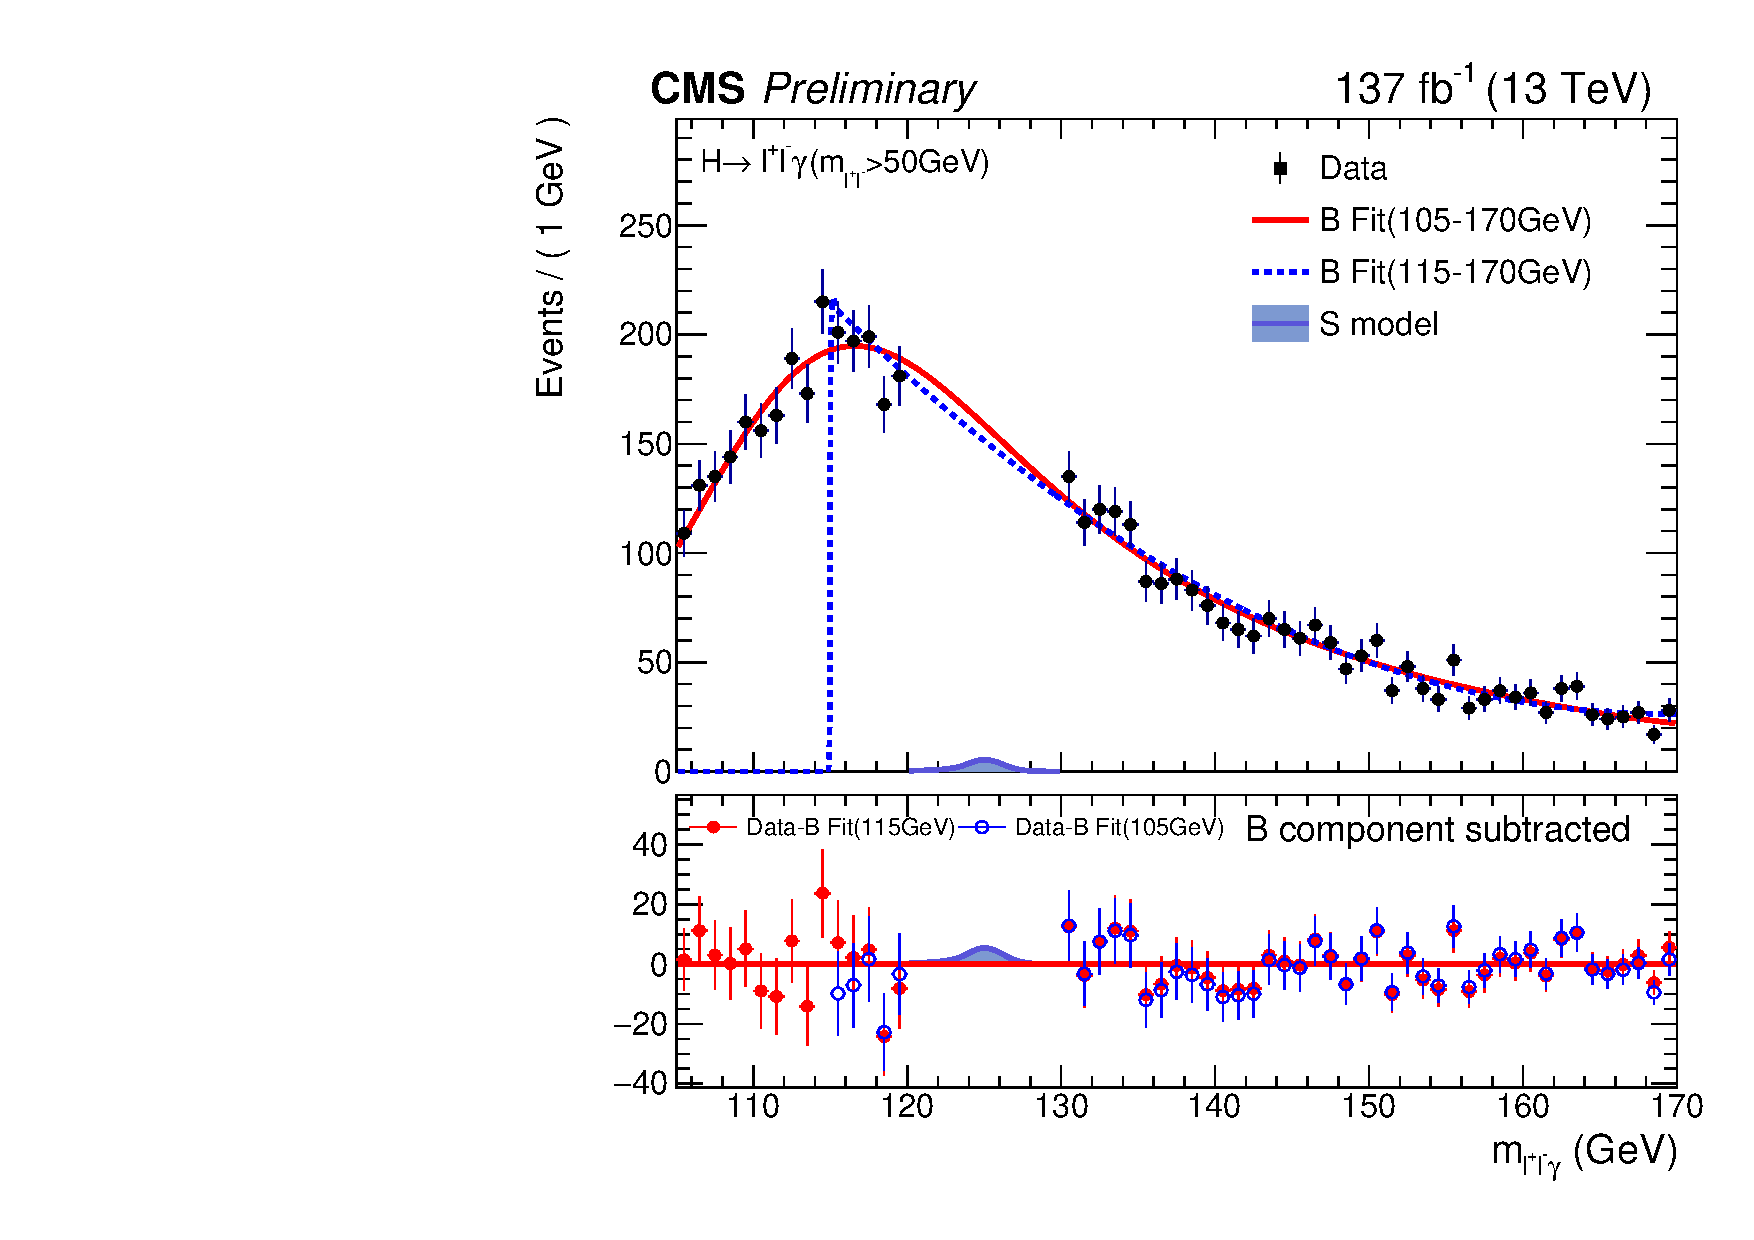
\includegraphics[width=0.33\textwidth]{fig/turnon_comparison/over_cat1_prefit_new.pdf}
        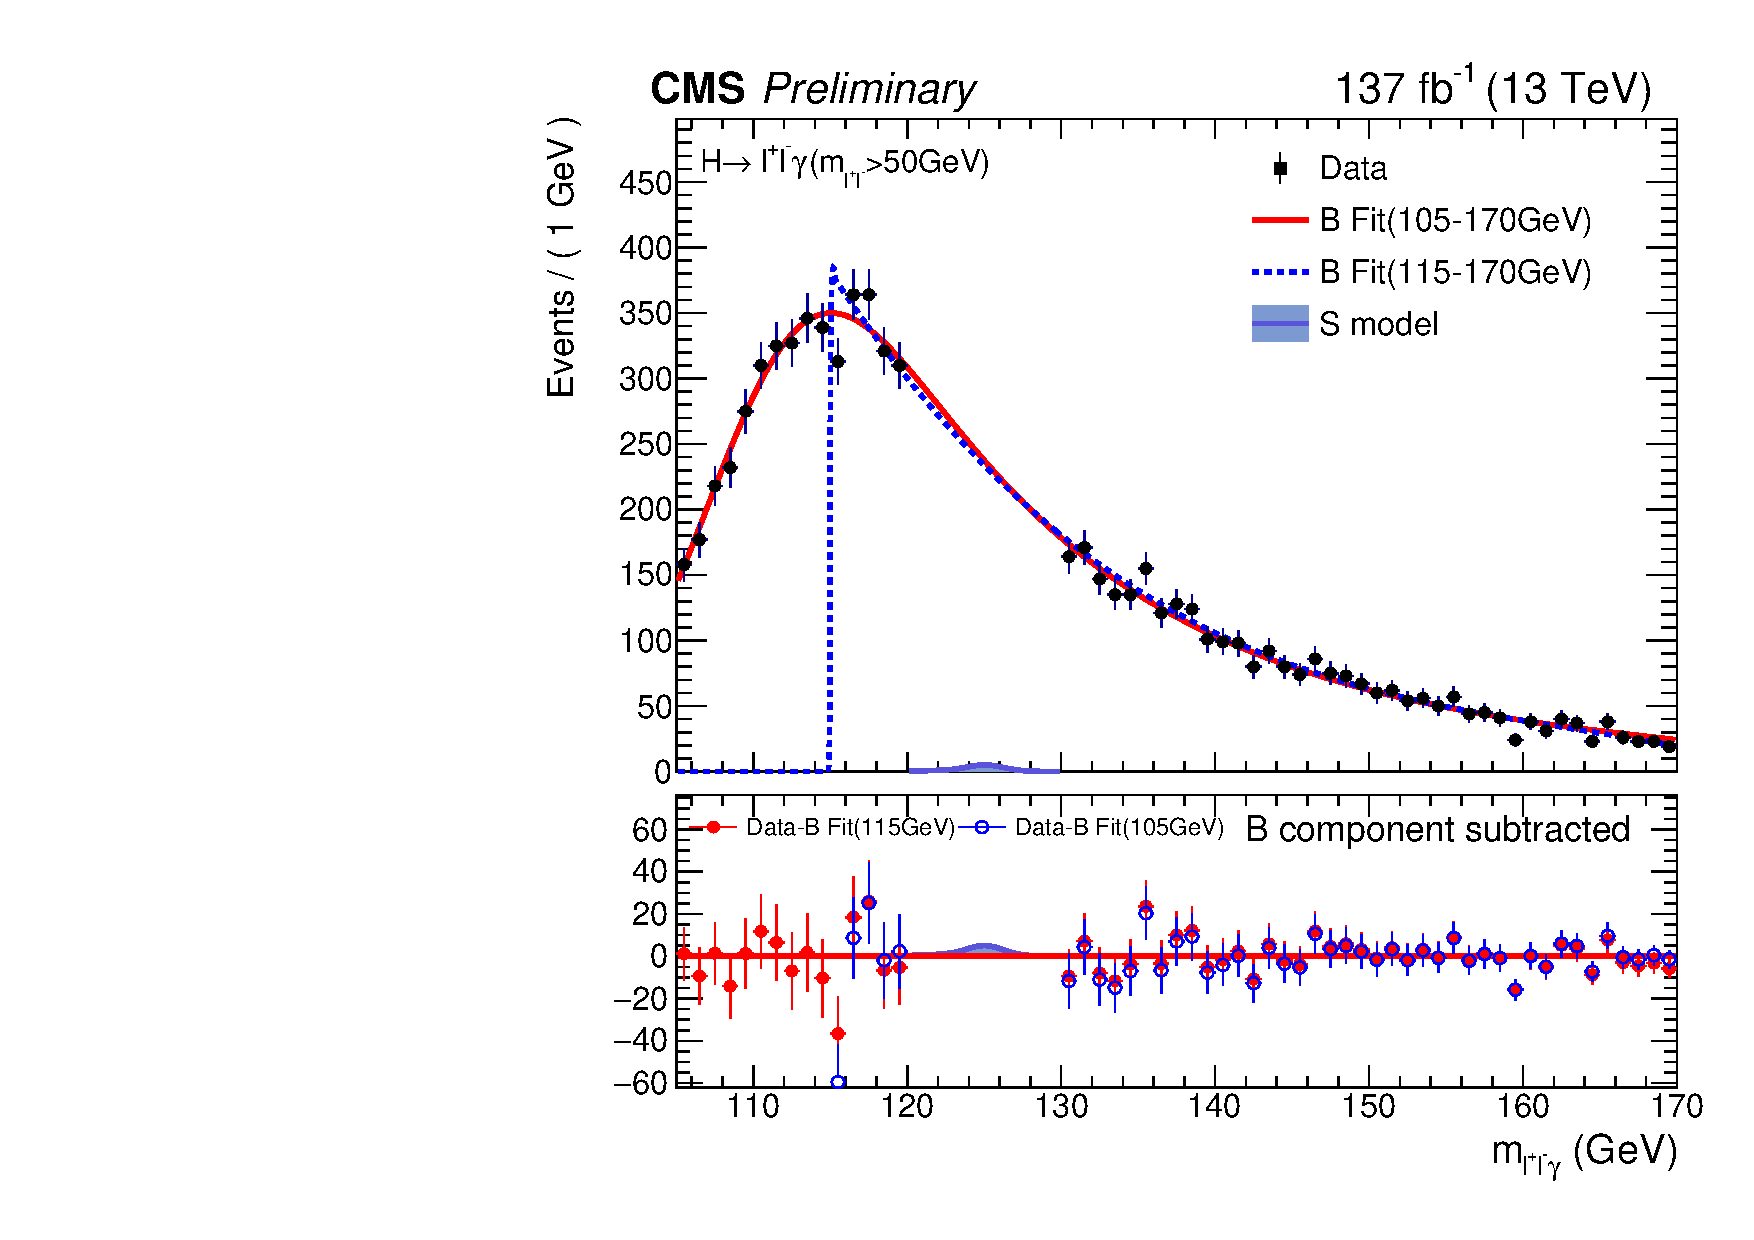
\includegraphics[width=0.33\textwidth]{fig/turnon_comparison/over_cat2_prefit_new.pdf}\\
        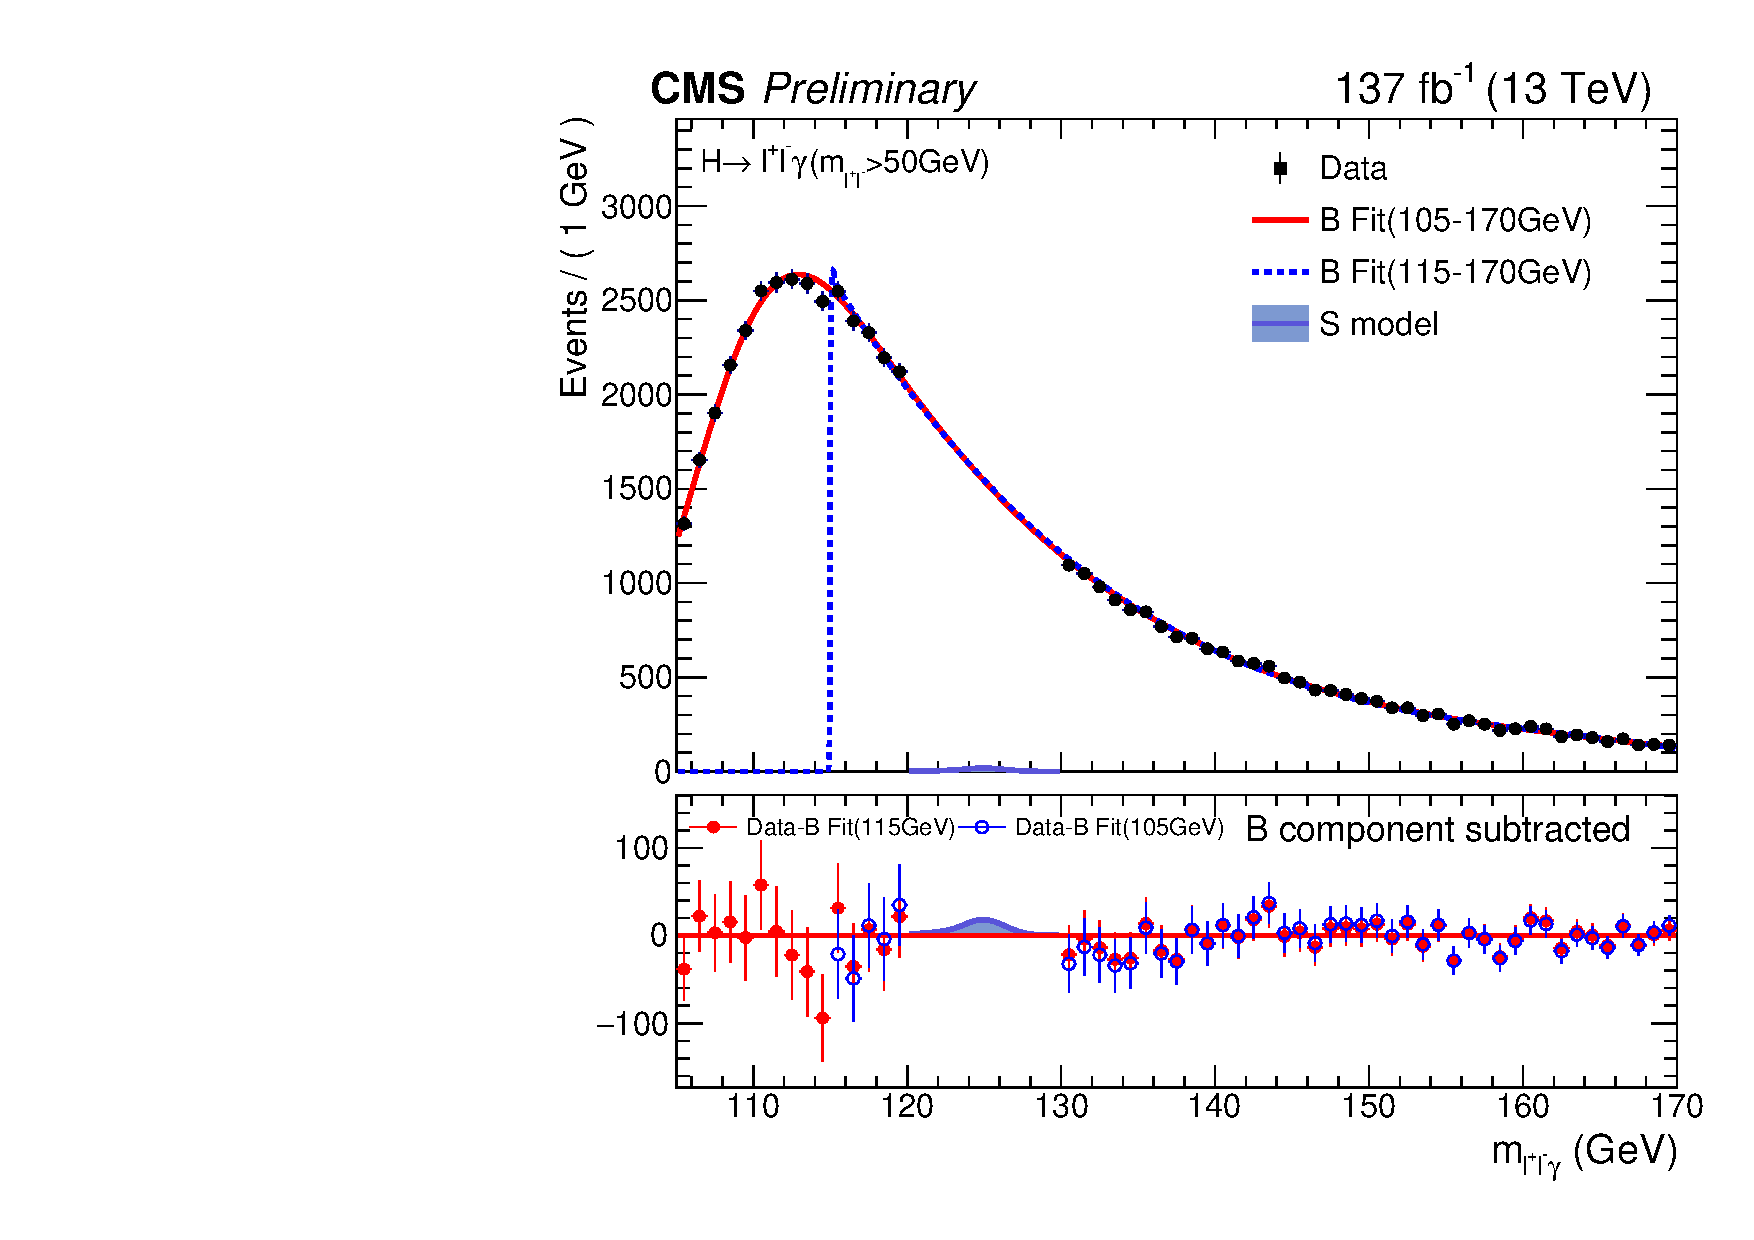
\includegraphics[width=0.33\textwidth]{fig/turnon_comparison/plot_cat3_prefit_new.pdf}
        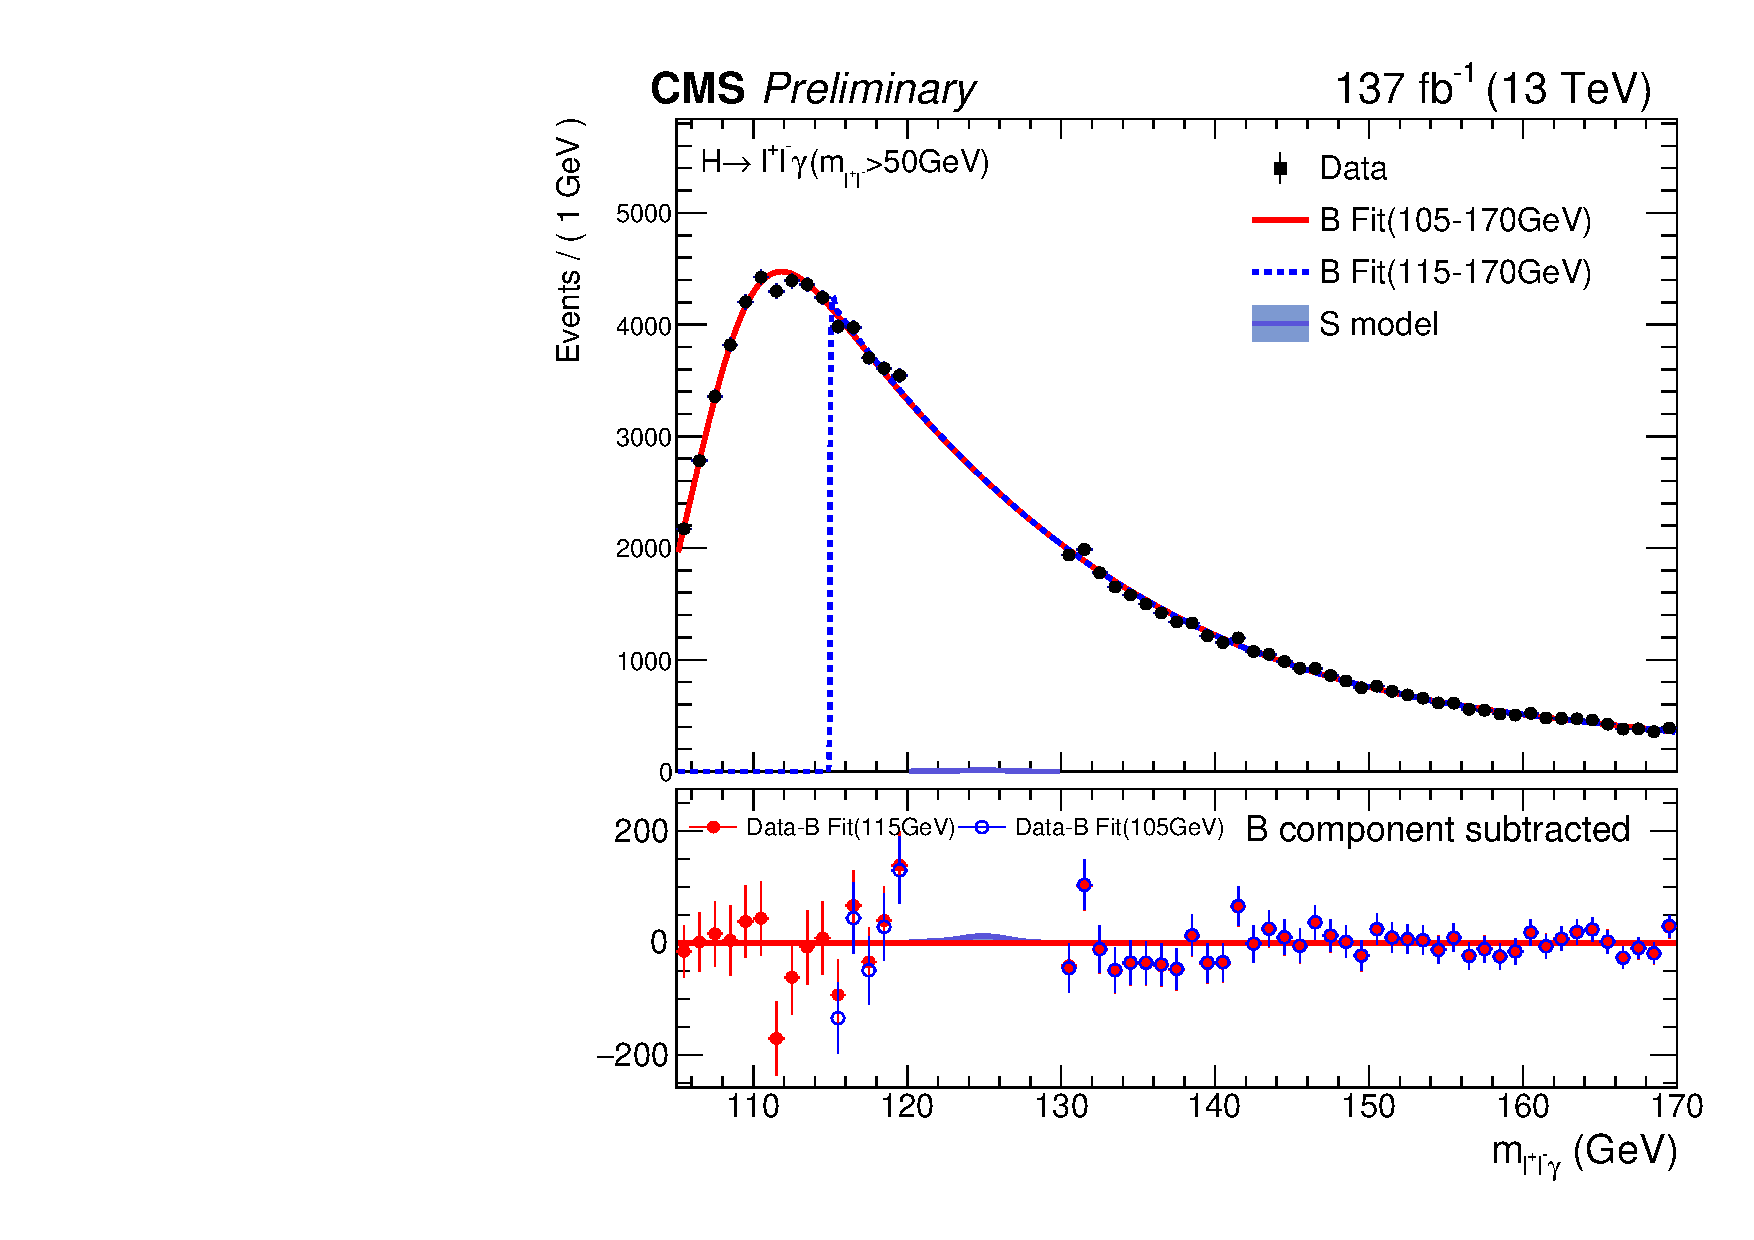
\includegraphics[width=0.33\textwidth]{fig/turnon_comparison/plot_cat4_prefit_new.pdf}\\
        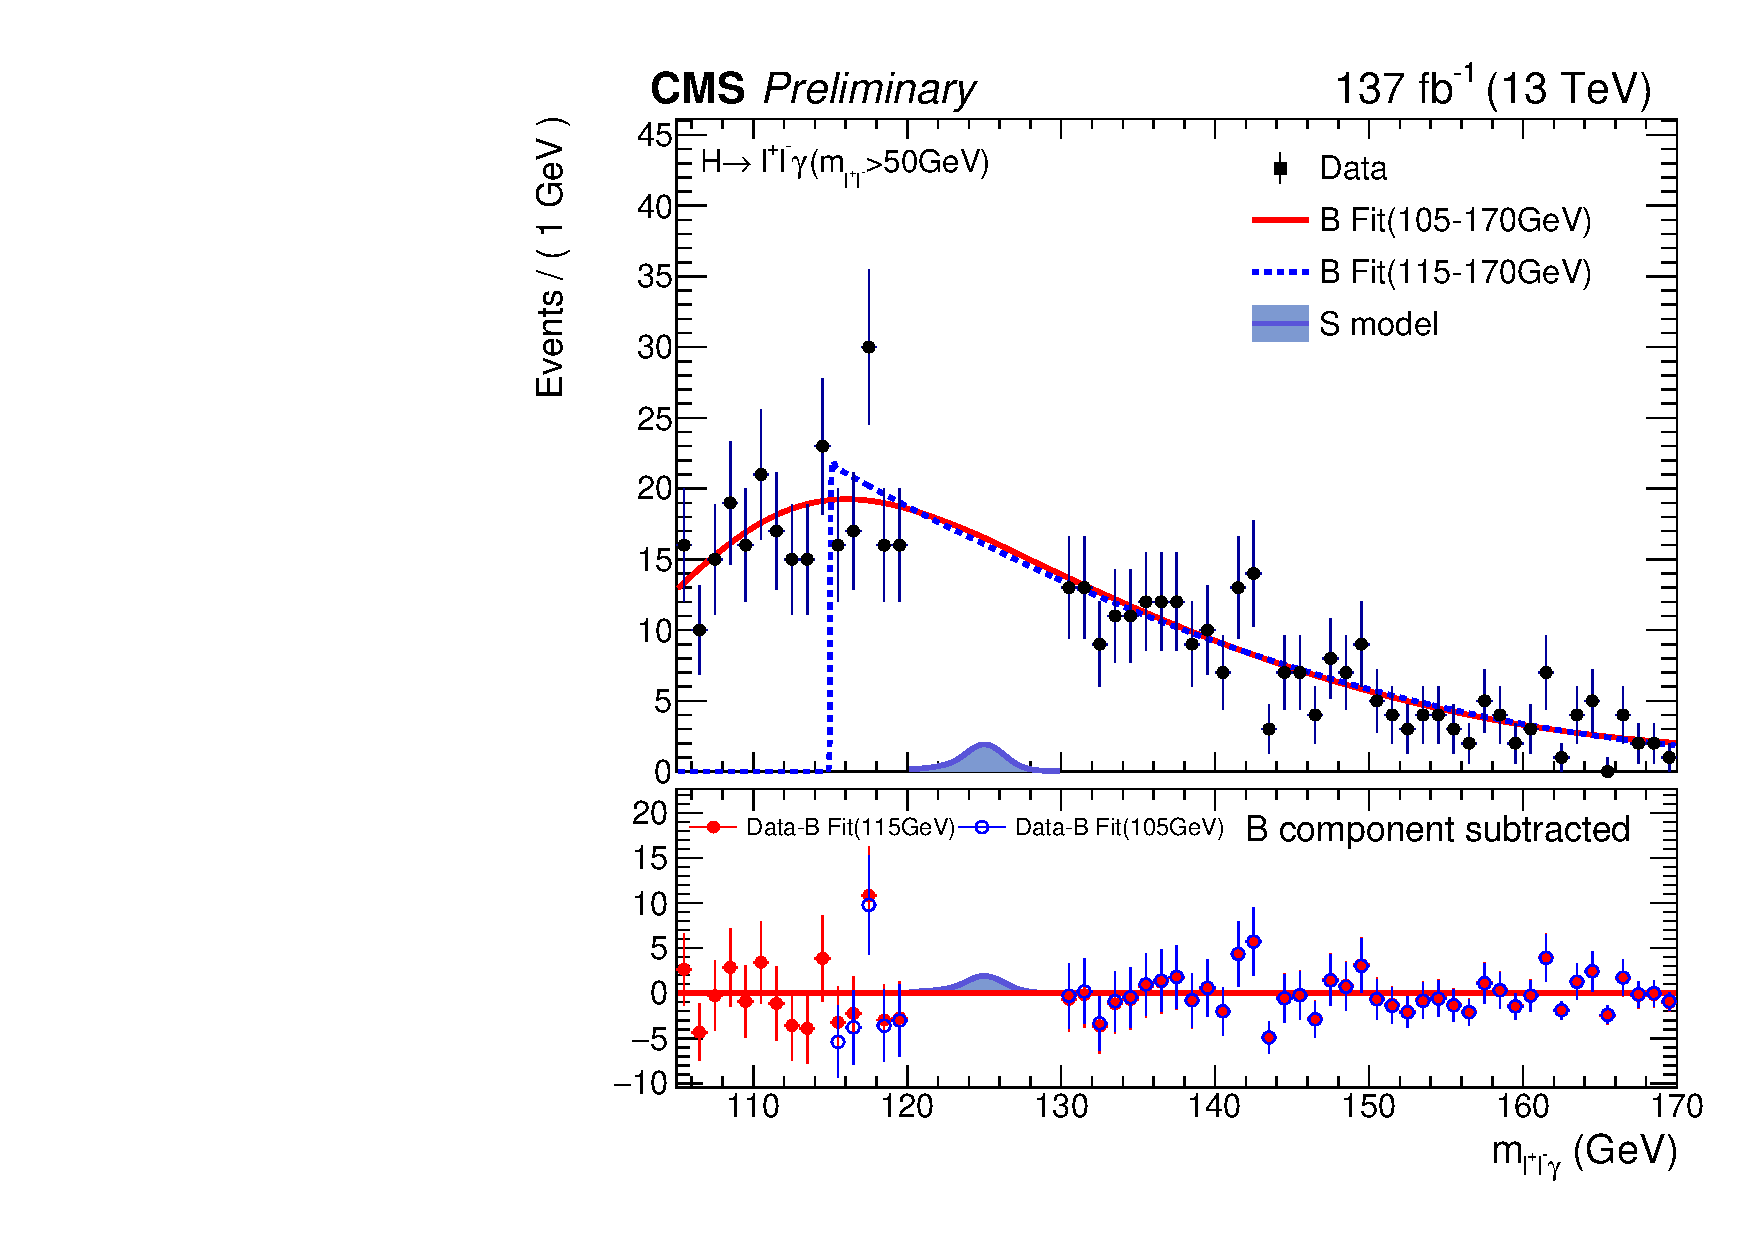
\includegraphics[width=0.33\textwidth]{fig/turnon_comparison/over_cat501_prefit_new.pdf}
        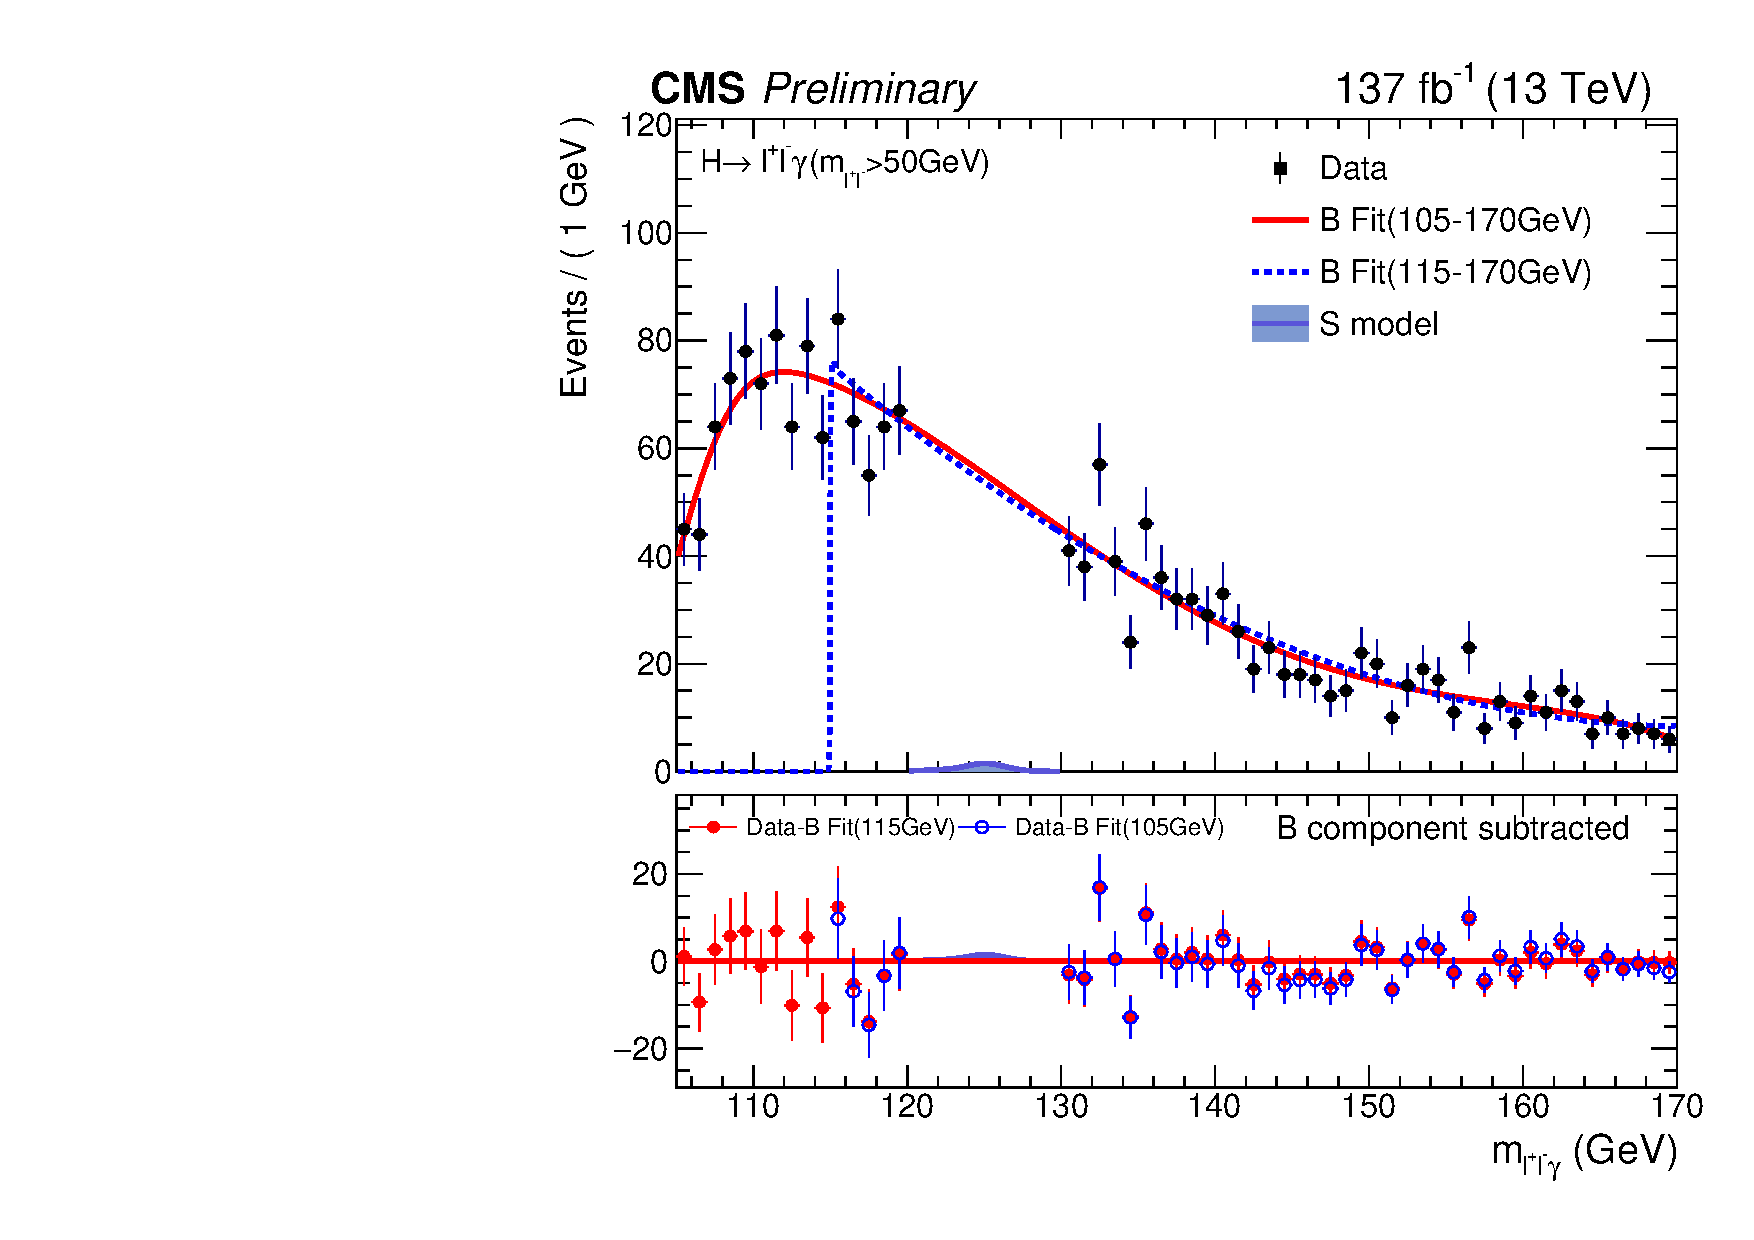
\includegraphics[width=0.33\textwidth]{fig/turnon_comparison/over_cat502_prefit_new.pdf}\\
        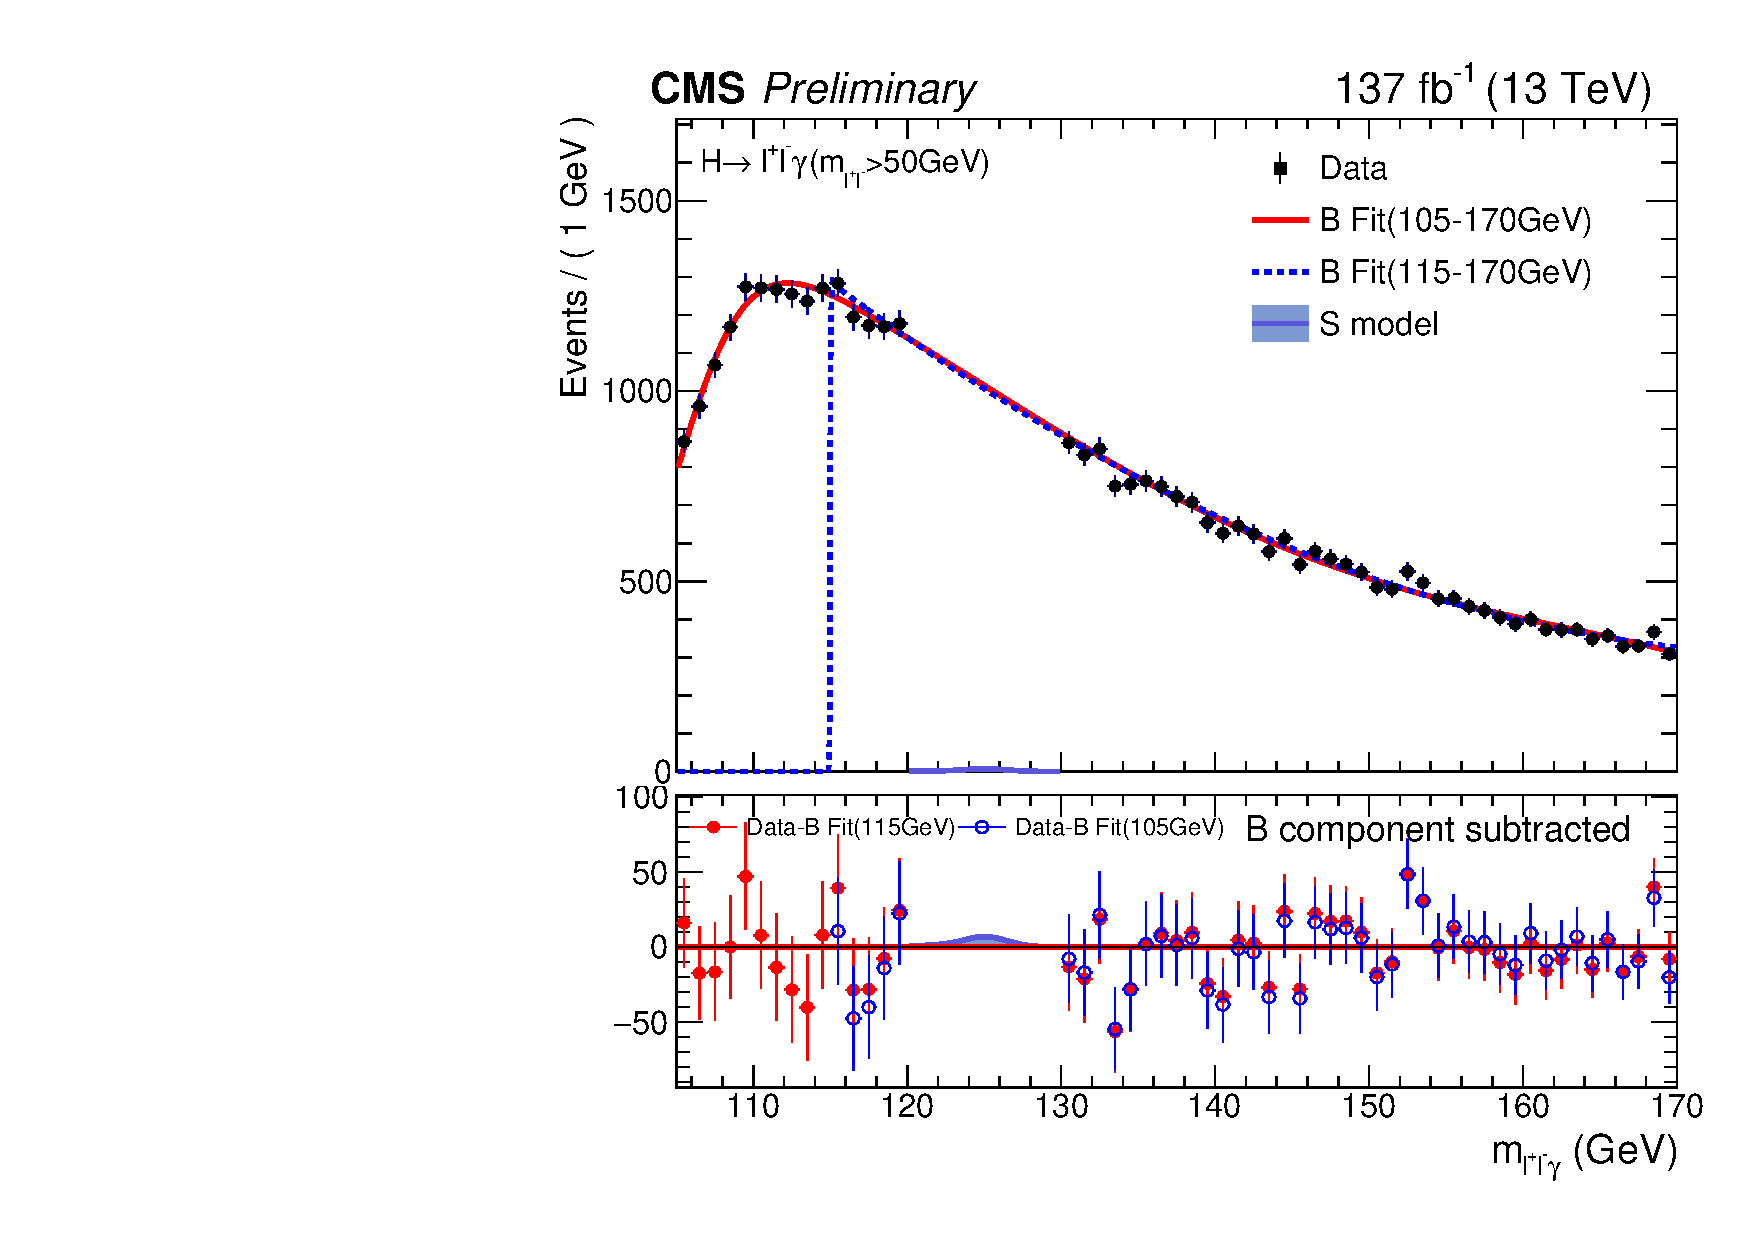
\includegraphics[width=0.33\textwidth]{fig/turnon_comparison/plot_cat503_prefit_new.pdf}
        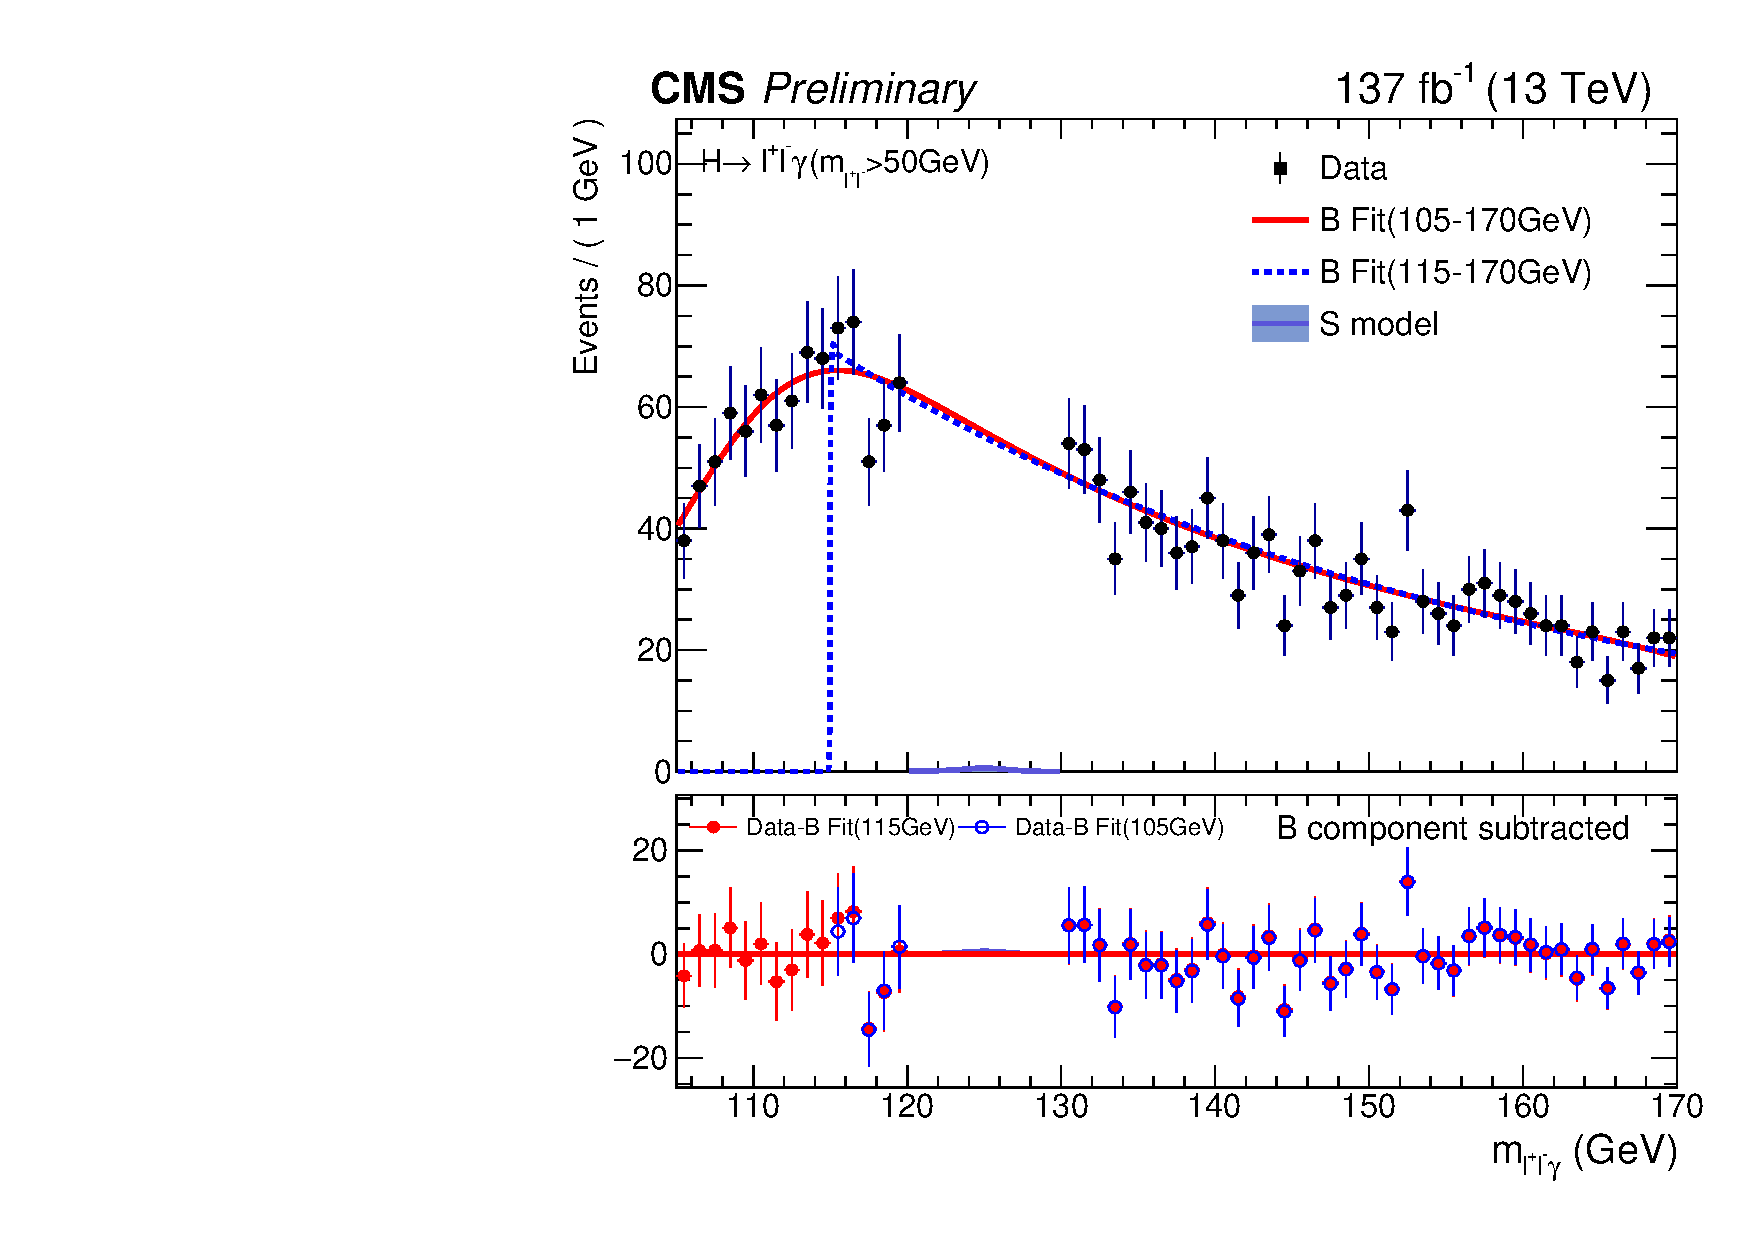
\includegraphics[width=0.33\textwidth]{fig/turnon_comparison/over_plot6789_prefit_new.pdf}
        \caption{Comparison of background fits with and without modeling the turn-on. 
        The top four plots correspond to the untagged categories, and the bottom four plots correspond to the dijet categories and lepton tag category.}
		\label{fig:compare_turnon_fits}
	\end{center}
\end{figure}

\subsection{Envelope Bias Studies}\label{sec:envelope_bias_studies}
Upon the selection of an initial envelope of PDFs to model the background in a 
given category of the analysis, a bias study is performed for that category. 
The principal goal of the bias study is to measure the bias and coverage of the 
full model, the envelope of functions, for different choices of the true 
underlying PDF. Of course, we do not know the true underlying PDF a priori, so 
we rely on the chi-squared and F-test probabilities used to construct the 
envelope to identify likely truth functions. In practice, this means that each 
individual PDF in the envelope is considered separately as a possible truth function
in our bias studies. There are several possible outcomes of the bias studies in each 
category. One outcome is that the bias is minimal and the coverage good for all 
truth functions. In this case, we accept the composition of the envelope as good 
for the analysis. Another possible outcome is that one or more truth functions is 
associated with a large (significantly greater than 14\%) bias or low 
(significantly less than 68\%) coverage. In this case, we can consider adding 
more functions to the envelope to increase the flexibility of the model, and then 
retry the bias study using the extended envelope. 

A more precise description of the bias study procedure follows. First, we generate 
a set of 1,000 toy datasets for a given truth function. The parameters of the truth 
function are fixed by fitting the data. Then, this PDF is used to generate the toys, 
with the same level of statistical uncertainty as the data
and assuming a true signal strength of zero (background only). Next, each toy is fit using 
the full envelope, where the index of the best fit function is profiled with the 
signal strength. In general, this means that different toys may be fit by different 
constituent PDFs within the envelope, and these PDFs may be different from the generating PDF. 
For each toy fit, we obtain a best fit signal strength $\hat{r}$ and a 68\% confidence interval
($\hat{r}_{down}$, $\hat{r}_{up}$). We define the pull for each toy as 
$pull = (\hat{r}-r_{true})/\sigma_{\hat{r}}$. In the background only case, $r_{true} = 0$. 
The uncertainty in the denominator accounts for
the assymetric error bars coming from the confidence interval. The pull distribution is expected
to be a unit Gaussian. We fit the pull distribution with a Gaussian, and the best fit mean 
value is taken to be the bias. The coverage is defined as the frequency with which zero falls
within the confidence interval ($\hat{r}_{down}$, $\hat{r}_{up}$). It is expected to be 
near 68\%. If overcoverage is observed, this implies the uncertainty in the signal strength may 
be overly conservative. Within a few percent of 68\%, this is acceptable. If undercoverage of 
a significant amount is observed, this implies a problem with the model, and may mean that 
the individual functions are biased or that the envelope should be made more flexible. 

The bias and coverage results for the final envelope in each category 
are shown in Tables \ref{tab:bias_cat1_m105-170} through \ref{tab:bias_cat6789_m105-170}. 
Note that in all categories except untagged 3, untagged 4, and dijet 3, the envelope functions 
are exactly those identified by the chi-squared and F-test probabilities previously described.
However, in untagged 3, untagged 4, and dijet 3, it was observed that the initial functions chosen 
by the chi-squared and F-test procedure showed large biases (greater than 20\%) and low coverages (less than 60\%) for 
certain truth functions. Therefore, the envelope was extended to include higher order Bernstein functions up 
to order 5 for each of these categories. The bias tables for these categories reflect the results for the final 
extended envelope. 

%For each choice of truth function, it is also useful to keep track of the frequency at which each 
%constituent PDF in the envelope is chosen by the fit. That is, what fraction of the toys is fit by
%each function. This can aid in detecting potential issues and interpreting bias. The frequency 
%heat maps in each category are shown in Figure \ref{fig:envelope_heatmaps_105_170}.

\begin{table}
	\caption{Bias and coverage results for each category.}
    \footnotesize
	\centering
    \begin{subtable}{\textwidth}
	    \centering
    \begin{tabular}{|c|cccccccc|} \hline
        \textbf{Generating PDF} & Exp1 & Pow1 & Lau1 & Lau2 & Lau3 & Lau4 & Bern2 & Bern3\\ \hline
        \textbf{Bias} & \tabincell{c}{-0.03\\$\pm$0.03}& \tabincell{c}{0.02\\$\pm$0.04}& \tabincell{c}{0.02\\$\pm$0.04}& \tabincell{c}{0.06\\$\pm$0.04}& \tabincell{c}{0.04\\$\pm$0.04}& \tabincell{c}{-0.09\\$\pm$0.04} &\tabincell{c}{-0.07\\$\pm$0.03} &\tabincell{c}{0.00\\$\pm$0.04}\\ 
        \textbf{Coverage} & 0.68 & 0.66 & 0.71 & 0.68 & 0.71 & 0.68 & 0.65 & 0.70\\ \hline
    \end{tabular}
    \caption{Untagged 1 bias and coverage results from the final envelope bias study.}
    \label{tab:bias_cat1_m105-170}
    \end{subtable}
    \vspace*{0.25 cm}
    \begin{subtable}{\textwidth}
        \footnotesize
        \centering
        \begin{tabular}{|c|ccccc|} \hline
            \textbf{Generating PDF} &Exp1 &Pow1 &Lau3 &Bern2 &Bern3\\ \hline
            \textbf{Bias} &\tabincell{c}{-0.10\\$\pm$0.04}&\tabincell{c}{-0.09\\$\pm$0.05} &\tabincell{c}{-0.27\\$\pm$0.04}& \tabincell{c}{-0.07\\$\pm$0.03} & \tabincell{c}{0.07\\$\pm$0.04}\\ 
            \textbf{Coverage} & 0.67 & 0.66 & 0.67 & 0.67 & 0.65\\ \hline
        \end{tabular}
        \caption{Untagged 2 bias and coverage results from the final envelope bias study.}
        \label{tab:bias_cat2_m105-170}
    \end{subtable}
    \vspace*{0.25 cm}
    \begin{subtable}{\textwidth}
        \footnotesize
        \centering
        \begin{tabular}{|c|ccccc|} \hline
            \textbf{Generating PDF} &Exp1 &Pow1 &Bern3&Bern4&Bern5\\ \hline
            \textbf{Bias} &\tabincell{c}{-0.05\\$\pm$0.04}&\tabincell{c}{-0.11\\$\pm$0.03}&\tabincell{c}{0.03\\$\pm$0.04}&\tabincell{c}{-0.02\\$\pm$0.03}&\tabincell{c}{0.27\\$\pm$0.04}\\ 
            \textbf{Coverage} & 0.67&0.67 & 0.70 &0.67 & 0.66\\ \hline
        \end{tabular}
        \caption{Untagged 3 bias and coverage results from the final envelope bias study.}
        \label{tab:bias_cat3_m105-170}
    \end{subtable}
    \vspace*{0.25 cm}
    \begin{subtable}{\textwidth}
        \footnotesize
        \centering
        \begin{tabular}{|c|cccc|} \hline
            \textbf{Generating PDF} &Exp3 &Bern3 &Bern4 &Bern5\\ \hline
            \textbf{Bias} &\tabincell{c}{-0.08\\$\pm$0.03} &\tabincell{c}{0.07\\$\pm$0.03} &\tabincell{c}{0.16\\$\pm$0.03} &\tabincell{c}{0.10\\$\pm$0.03}\\ 
            \textbf{Coverage} & 0.68 & 0.67 & 0.67 & 0.68\\ \hline
        \end{tabular}
        \caption{Untagged 4 bias and coverage results from the final envelope bias study.}
        \label{tab:bias_cat4_m105-170}
    \end{subtable}
    \vspace*{0.25 cm}
\begin{subtable}{\textwidth}
    \footnotesize
    \centering
    \begin{tabular}{|c|ccccccc|} \hline
        \textbf{Generating PDF} &Exp1 &Pow1 &Lau1 &Lau2 &Lau3 &Lau4 &Bern2\\ \hline
        \textbf{Bias} &\tabincell{c}{0.03\\$\pm$0.03} &\tabincell{c}{0.09\\$\pm$0.03} &\tabincell{c}{-0.02\\$\pm$0.04}&\tabincell{c}{-0.06\\$\pm$0.04} &\tabincell{c}{-0.02\\$\pm$0.03} &\tabincell{c}{0.02\\$\pm$0.03} &\tabincell{c}{-0.04\\$\pm$0.03}\\ 
        \textbf{Coverage} & 0.64 & 0.66 & 0.66 & 0.68 & 0.67 & 0.68 & 0.66\\ \hline
    \end{tabular}
    \caption{Dijet 1 bias and coverage results from the final envelope bias study.}
    \label{tab:bias_cat501_m105-170}
\end{subtable}
\vspace*{0.25 cm}
\begin{subtable}{\textwidth}
    \footnotesize
    \centering
    \begin{tabular}{|c|cccccccccc|} \hline
        \textbf{Generating PDF} &Exp1 &Pow1 &Pow3 &Lau2 &Lau3& Lau4&Bern2 &Bern3 &Bern4 & Bern5\\ \hline
        \textbf{Bias} & \tabincell{c}{-0.12\\$\pm$0.04} &\tabincell{c}{ -0.29\\$\pm$0.04} & \tabincell{c}{-0.14\\$\pm$0.04} & \tabincell{c}{-0.22\\$\pm$0.04} & \tabincell{c}{-0.16\\$\pm$0.04} & \tabincell{c}{-0.18\\$\pm$0.04} &\tabincell{c}{-0.06\\$\pm$0.04} &\tabincell{c}{-0.05\\$\pm$0.03} & \tabincell{c}{0.05\\$\pm$0.03} & \tabincell{c}{-0.13\\$\pm$0.03}\\ 
        \textbf{Coverage} & 0.67 & 0.65 & 0.68 & 0.66 & 0.66 & 0.67 & 0.68 & 0.64 & 0.67 & 0.65\\ \hline
    \end{tabular}
    \caption{Dijet 2 bias and coverage results from the final envelope bias study.}
    \label{tab:bias_cat502_m105-170}
\end{subtable}
%\newline
\vspace*{0.25 cm}
%\newline
\begin{subtable}{\textwidth}
    \footnotesize
    \centering
    \begin{tabular}{|c|cccccccccc|} \hline
        \textbf{Generating PDF} &Exp1 &Pow1 & Pow3 &Lau2 &Lau3 & Lau4 & Bern2 &Bern3 &Bern4 &Bern5\\ \hline
        \textbf{Bias} & \tabincell{c}{-0.12\\$\pm$0.03} & \tabincell{c}{-0.29\\$\pm$0.04} & \tabincell{c}{-0.14\\$\pm$0.04} &\tabincell{c}{-0.22\\$\pm$0.04} &\tabincell{c}{-0.16\\$\pm$0.03}&\tabincell{c}{-0.18\\$\pm$0.03} & \tabincell{c}{-0.06\\$\pm$0.03} & \tabincell{c}{-0.03\\$\pm$0.05} & \tabincell{c}{0.05\\$\pm$0.03} & \tabincell{c}{-0.13\\$\pm$0.03}\\ 
        \textbf{Coverage} & 0.67 & 0.65 & 0.68 & 0.67 & 0.66 & 0.67 & 0.68 & 0.64 & 0.67 & 0.65\\ \hline
    \end{tabular}
    \caption{Dijet 3 bias and coverage results from the final envelope bias study.}
    \label{tab:bias_cat503_m105-170}
\end{subtable}
%\newline
\vspace*{0.25 cm}
%\newline
\begin{subtable}{\textwidth}
    \footnotesize
    \centering
    \begin{tabular}{|c|ccccc|} \hline
        \textbf{Generating PDF} &Exp1 &Pow1 &Lau1 &Lau2 &Bern2\\ \hline
        \textbf{Bias} &  \tabincell{c}{-0.04\\$\pm$0.03} &  \tabincell{c}{0.05\\$\pm$0.03} &  \tabincell{c}{0.27\\$\pm$0.04} &  \tabincell{c}{0.03\\$\pm$0.03} & \tabincell{c}{-0.03\\$\pm$0.03}\\ 
        \textbf{Coverage} & 0.71 & 0.69 & 0.66 & 0.70 & 0.70\\ \hline
    \end{tabular}
    \caption{Lepton tag bias and coverage results from the final envelope bias study.}
    \label{tab:bias_cat6789_m105-170}
\end{subtable}
\end{table}






%\begin{figure}
%	\begin{center}
%        \includegraphics[width=0.35\textwidth]{fig/biasPlots/turnon_bias/turnonfit/fix_m105_170/heatmap_cat1.png}
%        \includegraphics[width=0.35\textwidth]{fig/biasPlots/turnon_bias/turnonfit/fix_m105_170/heatmap_cat2.png}\\
%        \includegraphics[width=0.35\textwidth]{fig/biasPlots/turnon_bias/turnonfit/fix_m105_170/heatmap_cat3.png}
%        \includegraphics[width=0.35\textwidth]{fig/biasPlots/turnon_bias/turnonfit/fix_m105_170/heatmap_cat4.png}\\
%        \includegraphics[width=0.35\textwidth]{fig/biasPlots/turnon_bias/turnonfit/fix_m105_170/heatmap_cat501.png}
%        \includegraphics[width=0.35\textwidth]{fig/biasPlots/turnon_bias/turnonfit/fix_m105_170/heatmap_cat502.png}\\
%        \includegraphics[width=0.35\textwidth]{fig/biasPlots/turnon_bias/turnonfit/fix_m105_170/heatmap_cat503.png}
%        \includegraphics[width=0.35\textwidth]{fig/biasPlots/turnon_bias/turnonfit/fix_m105_170/heatmap_cat6789.png}\\
%        \caption{Fit frequency heat maps for the functions chosen for the initial envelope.
%        The top four plots correspond to the untagged categories, and the bottom four plots correspond to the dijet categories and lepton tag category.}
%		\label{fig:envelope_heatmaps_105_170}
%	\end{center}
%\end{figure}

\subsection{Interpretation of Bias Study Results}
We now turn to the interpretation of the initial envelope bias studies. First, it can be seen that most 
categories show no signs of significant bias or undercoverage for any potential truth functions. 
Specifically, we see that the envelopes for categories untagged 1, untagged 4, and dijet 1
can immediately be accepted as good for the analysis. In untagged 2, untagged 3, dijet 2, dijet 3, and the lepton 
tag category, specific truth functions deserve a bit more scrutiny. 

In the untagged 2, dijet 2, dijet 3, and lepton tag categories, we observe slightly larger bias for the Laurent polynomial truth functions. 
From the heat map of the chosen functions, we can see the toys generated with Laurent functions are most often fit with 
Bernstein polynomials. Additionally, from the initial chi-squared probability results in Table \ref{tab:function_probs}, 
the Laurent functions give lower probabilities than the other functions in the envelope. 
This means that they are quite unlikely to be the actual truth function. From the likelihood scan with $\mu=1$ in 
Figure \ref{fig:func_scan_allcat_exp}, we also observe that the Laurent functions are not involved in the likelihood scan between 0 and 1.
This means that the Laurent family is irrevelant in the final background model. 
Given this consideration, along with the fairly good coverage for these 
Laurent functions, we expect the impact of these biases on the analysis to be negligible. A similar line of logic also applies to the 
case of the power law 1 truth function in categories dijet 2 and dijet 3. Again, we expect the impact of these biases to be negligible.

In untagged 3, we observe a small, but somewhat significant bias of 27\% for the truth function with falling spectrum
component Bernstein 5. In this case, we see that the coverage of 66\% is still quite good, only slightly below 68\%. 
Looking at the fit frequency heat map for this category, we see that this bias arises when the fit function is a 
lower order Bernstein polynomial. This type of behavior is expected. Generating with a higher order and fitting with a lower 
order within the same function family will usually yield some level of bias. This is less of a concern than a case in which one 
truth family shows a large bias when fit with a different family. Given the small size of the bias for a single truth 
function, and the fact that the behavior is somewhat expected for lower order fits within the Bernstein family, we expect 
the overall impact on the analysis to be negligible. Therefore, the untagged 3 envelope is also deemed fine for the analysis. 

